\subsection{半局部环的 Hausdorff 完备化}

命题 17。设 A 为交换环，\((\mathfrak{m}_{\lambda})_{\lambda \in L}\) 是 A 的一个理想族，各理想均不等于 A，并且当 \(\mathfrak{m}_{\lambda}\) 与 \(\mathfrak{m}_{\mu}\) 满足 \(\lambda \neq \mu\) 时二者互素。对于任意一个族 \(s = (s(\lambda))_{\lambda \in L}\)，其元素为 \(\geqslant 0\) 的整数且具有有限支撑，置 \(\mathfrak{a}_{s} = \bigcap_{\lambda \in L} \mathfrak{m}_{\lambda}^{s(\lambda)}\)（它等于所有 \(\mathfrak{m}_{\lambda}^{s(\lambda)}\) 的乘积，其中的 \(\lambda\) 满足 \(s(\lambda) \neq 0\)；参见~第二章，第 1 节，第 2 号，命题 3 和 5）；\(\mathfrak{a}_{s}\) 构成关于与 A 的环结构相容的拓扑 \(\mathcal{T}\) 的 0 的邻域基本系；设 \(\hat{\mathbf{A}}\) 为 A 关于此拓扑的 Hausdorff 完备化。另一方面，对于所有 \(\lambda \in L\)，令 \(\mathbf{A}_{\lambda}\) 为赋予 \(\mathfrak{m}_{\lambda}\)-进拓扑的环 A，并令 \(\hat{\mathbf{A}}_{\lambda}\) 为其 Hausdorff 完备化。若 \(u: \mathbf{A} \to \prod_{\lambda \in L} \mathbf{A}_{\lambda}\) 表示对角同态，则 \(u\) 连续，且相应的同态 \(\hat{u}\)：

\[
\hat {\mathbf {A}} \rightarrow \left(\prod_ {\lambda \in \mathbf {L}} \mathbf {A} _ {\lambda}\right) ^ {\wedge} = \prod_ {\lambda \in \mathbf {L}} \hat {\mathbf {A}} _ {\lambda}
\]

（一般拓扑学，第三章，第 6 节，第 5 号以及第二章，第 3 节，第 9 号，命题 18 的推论 2）是一个拓扑环同构。

第一个断言由一般拓扑学第三章，第 6 节，第 3 号，例 3 得出。置 \(\mathbf{B} = \prod_{\lambda \in \mathbf{L}} \mathbf{A}_{\lambda}\)；由于 \(\mathbf{A}\) 上的拓扑比每个 \(m_{\lambda}\)-进拓扑都细，映射 \(\mathrm{pr}_{\lambda} \circ u\) 连续，因而 \(u\) 连续。此外，\(u(a_s)\) 是 \(\Delta\)（\(\mathbf{B}\) 的对角线）与开集 \(\bigcap_{\lambda \in \mathbf{L}} \mathrm{pr}_{\lambda}^{-1}(m_{\lambda}^{s(\lambda)})\)（\(\mathbf{B}\) 中）的交；由此可知，\(u\) 是从加法群 \(\mathbf{A}\) 到 \(\mathbf{B}\) 的严格态射，其像为 \(\Delta\)。现在 \(\Delta\) 在 \(\mathbf{B}\) 中稠密。事实上，设 \(b = (a_{\lambda})_{\lambda \in \mathbf{L}}\) 是 \(\mathbf{B}\) 的一个元素；\(b\) 在 \(\mathbf{B}\) 中的每个邻域都包含形如 \(b + \mathbf{V}\) 的集合，其中 \(\mathbf{V} = \bigcap_{\lambda \in \mathbf{L}} \mathrm{pr}_{\lambda}^{-1}(m_{\lambda}^{s(\lambda)})\)，而 \(s = (s(\lambda))_{\lambda \in \mathbf{L}}\) 是一个具有有限支撑的、由整数 \(\geqslant 0\) 构成的族。由于 \(m_{\lambda}^{s(\lambda)}\) 两两互素（第二章，第 1 节，第 2 号，命题 3），存在 \(x \in \mathbf{A}\)，使得 \(x \equiv a_{\lambda}\)（模 \(m_{\lambda}^{s(\lambda)}\)）对所有 \(\lambda\) 都成立（同上，命题 5），从而 \((b + \mathbf{V}) \cap \Delta \neq \varnothing\)。于是群 \(\mathbf{B}/\Delta\) 的 Hausdorff 完备化为 \(\{0\}\)；将第 12 号的引理 2 应用于正合列 \(0 \to \mathbf{A} \xrightarrow{u} \mathbf{B}, \mathbf{A} \xrightarrow{u} \mathbf{B} \to \mathbf{B}/\Delta\)，可见 \(\hat{u}\) 是将 \(\hat{\mathbf{A}}\) 同构到 \(\hat{\mathbf{B}}\) 的同构。

推论。设 A 为主理想整环，P 为 A 的极端元代表系（代数，第七章，第 1 节，第 3 号）。A 上使 A 的 \(\neq0\) 理想构成 0 的邻域基本系、且与 A 的环结构相容的拓扑是 Hausdorff 的；A 关于此拓扑的完备化典范同构于 A 关于 \(\pi\)-进拓扑的完备化的乘积，其中 \(\pi\) 遍历 P。

主理想 \((\pi)\)（其中 \(\pi \in P\)）是极大的且彼此不同，因而互素；我们已经看到（第 12 号，例 3），\(\pi\)-进拓扑是 Hausdorff 的，所以命题 17 的叙述中定义的拓扑也是 Hausdorff 的，因为它比每个 \(\pi\)-进拓扑都细。

将命题 17 的推论应用于 A = Z 时，我们以 \(\hat{Z}\) 表示 Z 关于使 Z 的所有 \(\neq0\) 理想构成 0 的邻域基本系的拓扑的完备化；这个环同构于 p-进整数环的乘积 \(\prod_{p\in P}Z_{p}\)，其中 P 是素数集。

\textbf{注}\par

\begin{enumerate}
\def\labelenumi{(\arabic{enumi})}
\item
  显然，在命题 17 的条件下，拓扑 \(\mathcal{T}\) 是各 \(m_{\lambda}\)-进拓扑在 \(\mathbf{A}\) 上的上确界。
\item
  \(\mathfrak{a}\) 是 \(\prod_{\lambda \in L} \hat{\mathbf{A}}_{\lambda}\) 的每个闭理想，都等于其投影 \(\mathfrak{a}_{\lambda} = \operatorname{pr}_{\lambda}(\mathfrak{a})\) 的乘积，而这些投影是 \(\hat{\mathbf{A}}_{\lambda}\) 中的闭理想；因为 \(\hat{\mathbf{A}}_{\lambda}\) 典范地识别为闭理想 \(\mathbf{A}_{\lambda}'\)，它是 \(\prod_{\lambda} \hat{\mathbf{A}}_{\lambda}\) 的闭理想，并且 \(\mathfrak{a}_{\lambda}\) 识别为 \(\mathfrak{a} \cap \mathbf{A}_{\lambda}'\)（代数，第一章，第 8 节，第 10 号，命题 6），\(\mathfrak{a}_{\lambda}\) 的和在乘积 \(\prod_{\lambda} \mathfrak{a}_{\lambda}\) 中稠密（一般拓扑学，第三章，第 2 节，第 9 号，命题 25），而后者在 \(\prod_{\lambda} \hat{\mathbf{A}}_{\lambda}\) 中闭，由此得到所述断言。
\end{enumerate}

命题 18。设 A 为交换环，\((\mathfrak{m}_i)_{1 \leqslant i \leqslant q}\) 是 A 的有限个互不相同的极大理想组成的族，r 是乘积理想 \(\mathfrak{m}_1\mathfrak{m}_2 \ldots \mathfrak{m}_q = \mathfrak{m}_1 \cap \mathfrak{m}_2 \cap \cdots \cap \mathfrak{m}_q\)，S 是乘性子集 \(\bigcap_{i=1}^{q} (\mathbf{A} - \mathfrak{m}_i)\)。赋予 A r-进拓扑，赋予环 \(\mathbf{B} = \mathbf{S}^{-1}\mathbf{A}\) 以 rB-进拓扑，并赋予每个局部环 \(\mathbf{A}_{\mathfrak{m}_i}\) 以 \((\mathfrak{m}_i\mathbf{A}_{\mathfrak{m}_i})\)-进拓扑。令 \(u: \mathbf{A} \to \mathbf{B}\)、\(v_i: \mathbf{B} \to \mathbf{A}_{\mathfrak{m}_i}\) 为典范同态（第二章，第 2 节，第 1 号，命题 2 的推论 2），令 \(v\) 为同态 \((v_i): \mathbf{B} \to \prod_{i=1}^{q} \mathbf{A}_{\mathfrak{m}_i}\)。同态 \(u\) 和 \(v\) 连续，相应的同态 \(\hat{u}: \hat{\mathbf{A}} \to \hat{\mathbf{B}}\) 和 \(\hat{v}: \hat{\mathbf{B}} \to \prod_{i=1}^{q} (\mathbf{A}_{\mathfrak{m}_i})^{\wedge}\) 是拓扑环同构。

\(m_{i} \cap S = \varnothing\)（\(1 \leqslant i \leqslant q\)），所以 B 的理想 \(m_{i}' = m_{i}B\) 是极大的（第二章，第 2 节，第 5 号，命题 11），且

\[
\mathfrak {r B} = \mathfrak {m} _ {1} ^ {\prime} \cap \mathfrak {m} _ {2} ^ {\prime} \cap \dots \cap \mathfrak {m} _ {q} ^ {\prime}
\]

(第二章，第 2 节，第 4 号）；最后，\(\mathbf{B}_{\mathfrak{m}_i'} = \mathbf{A}_{\mathfrak{m}_i}\) 在一个典范同构下成立（第二章，第 2 节，第 5 号，命题 11）。由于 \(\bar{u}^{-1}(\mathfrak{rB}) = \mathfrak{r}\)，且 \(\bar{v}_i^{-1}(m_i\mathbf{A}_{\mathfrak{m}_i}) \supset \mathfrak{rB}\)，\(u\) 和 \(v\) 连续。因此只需证明：

\[
w = v \circ u: \mathrm{A} \rightarrow \prod_ {i = 1} ^ {q} \mathrm{A} _ {\mathfrak {m} _ {i}},
\]

\(\hat{w}\) 是 \(\hat{\mathbf{A}}\) 到 \(\prod_{i=1}^{q} \hat{\mathbf{A}}_{m_i}\) 上的同构，因为将此结果应用于 B 和 \(m_i'\) 将表明 \(\hat{v}\) 是同构，因而 \(\hat{u}\) 也是同构。注意，每个 \(m_i\) 的幂的乘积都包含 r 的某个幂，所以 r-进拓扑是各 \(m_i\)-进拓扑的上确界；此外，若 \(A_i\) 表示

\[
\mathfrak {m} _ {i} \text {-adic}
\]

\[
\phi : \mathrm{A} \rightarrow \prod_ {i = 1} ^ {q} \mathrm{A} _ {i}
\]

\(\hat{\phi}:\hat{\mathbf{A}}\to \prod_{i = 1}^{q}\hat{\mathbf{A}}_i\) 是一个同构（命题 17）。于是问题归结为证明：若 \(u_{i}:\mathbf{A}_{i}\rightarrow \mathbf{A}_{m_{i}}\) 是典范映射，则 \(\hat{u}_i\colon \hat{\mathbf{A}}_i\to \hat{\mathbf{A}}_{m_i}\) 是同构。现在，对所有 \(n\)，映射

\[
u _ {i, n} \colon \mathrm{A} / \mathfrak {m} _ {i} ^ {n} \rightarrow \mathrm{A} _ {\mathfrak {m} _ {i}} / \mathfrak {m} _ {i} ^ {n} \mathrm{A} _ {\mathfrak {m} _ {i}}
\]

由 \(u_{i}\) 取商得到的映射是同构（第二章，第 3 节，第 3 号，命题 9）；我们的断言由以下事实得出：\(\hat{\mathbf{A}}_i\)（分别为 \(\hat{\mathbf{A}}_{\mathfrak{m}_i}\)）是离散环 \(\mathbf{A} / \mathfrak{m}_i^n\)（分别为 \(\mathbf{A}_{\mathfrak{m}_i} / \mathfrak{m}_i^n \mathbf{A}_{\mathfrak{m}_i}\)）的逆极限（参见~第 6 号）。

注（3）。我们看到，一个整环 A 的 Hausdorff 完备化 \(\hat{A}\) 可能含有非零的零因子。

命题 19。设 A 为交换环，m 为 A 的极大理想。A 关于 m-进拓扑的 Hausdorff 完备化 \(\hat{\mathbf{A}}\) 是一个局部环，其极大理想为 \(\hat{\mathfrak{m}}\)。

若 \(\mathfrak{a} = \bigcap_{k\geqslant 1}\mathfrak{m}^k\)，则 \(\hat{\mathbf{A}}\) 是 Hausdorff 环 \(\mathbf{A} / \mathfrak{a}\)（与 \(\mathbf{A}\) 相伴）的完备化；又由于 \(\mathfrak{m} / \mathfrak{a}\) 是 \(\mathbf{A} / \mathfrak{a}\) 中的极大理想，我们可设 \(\mathbf{A}\) 关于 \(\mathfrak{m}\)-进拓扑是 Hausdorff 的。由于 \(\mathbf{A} / \mathfrak{m}\) 与 \(\hat{\mathbf{A}} /\hat{\mathfrak{m}}\) 是同构环（第 12 号，公式（21）），\(\hat{\mathfrak{m}}\) 是 \(\hat{\mathbf{A}}\) 的极大理想。由于 \(\hat{\mathbf{A}}\) 上的拓扑由滤过 \((\mathfrak{m}^n)^{\wedge}\) 定义（第 12 号），命题将由下述引理推出：

引理 3。设 A 为完备的 Hausdorff 拓扑环，且其中存在一个由 A 的加法子群组成的 0 的邻域基本系 \(\mathfrak{S}\)。

\begin{enumerate}
\def\labelenumi{(\roman{enumi})}
\item
  对于所有 \(x \in \mathbf{A}\) 满足 \(\lim_{n \to \infty} x^n = 0\)，\(1 - x\) 在 \(\mathbf{A}\) 中可逆，且其逆等于 \(\sum_{n=0}^{\infty} x^n\)。
\item
  设 \(\mathfrak{a}\) 是 A 的一个双边理想，满足 \(\lim x^n = 0\) 对所有 \(x \in \mathfrak{a}\) 都成立。A 的元素 y 可逆的充要条件是其模 a 的类在 A/a 中可逆；特别地，a 包含于 A 的 Jacobson 根中。
\end{enumerate}

(i) 由于

\[
(1 - x) (1 + x + \dots + x ^ {n}) = (1 + x + \dots + x ^ {n}) (1 - x) = 1 - x ^ {n + 1},
\]

问题归结为证明通项为 \(x^{n}\) 的级数在 A 中收敛；现在，根据假设，对于 A 中 0 的每个邻域 \(V \in \mathfrak{S}\)，存在整数 p \textgreater{} 0，使得 \(x^{n} \in V\) 对所有 \(n \geqslant p\) 都成立。于是

\[
x ^ {p} + x ^ {p + 1} + \dots + x ^ {q} \in \mathbf {V}
\]

对所有 \(q \geqslant p\) 都成立，而我们的断言随后由柯西判别法得出（一般拓扑学，第三章，第 5 节，第 2 号，定理 1）。

\begin{enumerate}
\def\labelenumi{(\roman{enumi})}
\setcounter{enumi}{1}
\tightlist
\item
  假设存在 \(y' \in A\)，使得 \(yy' \equiv 1 \pmod{a}\) 且 \(y'y \equiv 1 \pmod{a}\)。由 (i)，关于 \(a\) 的假设蕴含 \(yy'\) 和 \(y'y\) 在 \(A\) 中可逆，因而 \(y\) 在 \(A\) 中可逆。特别地，对每个 \(x \in a\)，\(1 - x\) 在 \(A\) 中可逆；又由于 \(a\) 是 \(A\) 的双边理想，它包含于 \(A\) 的 Jacobson 根中（代数，第八章，第 6 节，第 3 号，定理 1）。
\end{enumerate}

既已证明此引理，只需将其应用于拓扑环 \(\hat{\mathbf{A}}\) 及理想 \(\hat{\mathfrak{m}}\)，因为对于所有 \(x \in \hat{\mathfrak{m}}\)，都有 \(x^n \in (\hat{\mathfrak{m}})^n \subset (\mathfrak{m}^n)^\wedge\)，所以序列 \((x^n)\) 趋于 0。

若取 A = Z，则 Z 的每个极大理想都形如 pZ，其中 p 为素数。于是 p-进数环 \(Z_{p}\) 是一个局部环，其极大理想为 \(pZ_{p}\)（命题 16 的推论 2），其剩余域同构于 \(Z/pZ = F_{p}\)；而 \(\mathbf{Z}_{(p)}\) 赋予 \(pZ_{(p)}\)-进拓扑后，可识别为 \(Z_{p}\) 的一个包含 Z 的拓扑子环。

推论。设 A 为半局部环（第二章，第 3 节，第 5 号），\(\mathfrak{m}_i\) 为其互不相同的极大理想（\(1 \leqslant i \leqslant q\)），且

\[
\mathfrak {r} = \mathfrak {m} _ {1} \cap \mathfrak {m} _ {2} \cap \dots \cap \mathfrak {m} _ {q}
\]

它的 Jacobson 根。Hausdorff 完备化 \(\hat{\mathbf{A}}\) 是 \(\mathbf{A}\) 关于 \(\mathfrak{r}\)-进拓扑的完备化，是一个半局部环，典范同构于乘积 \(\prod_{i=1}^{q} \hat{\mathbf{A}}_{\mathfrak{m}_i}\)，其中 \(\hat{\mathbf{A}}_{\mathfrak{m}_i}\) 是局部环 \(\mathbf{A}_{\mathfrak{m}_i}\) 关于 \((\mathfrak{m}_i\mathbf{A}_{\mathfrak{m}_i})\)-进拓扑的 Hausdorff 完备化环。

\section{Noether 环上的 m-进拓扑}

本段所考虑的所有滤过均假定为穷竭的。

\subsection{好滤过}

设 A 为滤过交换环，E 为滤过 A-模，\((A_{n})\) 和 \((E_{n})\)

分别是 A 与 E 的滤过；设 \(A_{0} = A\)。在多项式环 A{[}X{]} 中，集合 \(A' = \sum_{n \geqslant 0} A_{n} X^{n}\) 是一个 N 型分次子 A-代数；子群 \(E' = \sum_{n \geqslant 0} E_{n} \otimes_{A} A X^{n}\)（属于 \(E \otimes_{A} A[X]\)）是一个 N 型分次 \(A'\)-模，因为

\[
\mathbf {A} _ {m} \mathbf {X} ^ {m} (\mathrm{E} _ {n} \otimes_ {\mathbf {A}} \mathbf {A X} ^ {n}) \subset (\mathbf {A} _ {m} \mathrm{E} _ {n} \otimes_ {\mathbf {A}} \mathbf {A X} ^ {m + n}) \subset \mathrm{E} _ {m + n} \otimes_ {\mathbf {A}} \mathbf {A X} ^ {m + n}.
\]

定义 1。设 A 为交换环，m 为 A 的理想，E 为 A-模，\((\mathrm{E}_{n})\) 是加法群 E 上由 E 的子模组成的一个滤过。若满足以下条件，则称滤过 \((\mathrm{E}_{n})\) 为 m-好：

\begin{enumerate}
\def\labelenumi{(\arabic{enumi})}
\item
  \(\mathfrak{m}\mathrm{E}_n\subset \mathrm{E}_{n + 1}\) 对所有 \(n\in \mathbf{Z}\) 都成立；
\item
  存在整数 \(n_0\)，使得 \(\mathfrak{m}\mathrm{E}_n = \mathrm{E}_{n+1}\) 对 \(n \geqslant n_0\) 成立。
\end{enumerate}

于是由 \(q\) 归纳可得，\(\mathfrak{m}^q\mathrm{E}_n = \mathrm{E}_{n + q}\) 对 \(n \geqslant n_0\)、\(q \geqslant 1\) 成立。注意，若 A 赋予 m-进滤过，条件（1）意味着滤过 \((\mathrm{E}_n)\) 与 E 上的 A-模结构相容。显然，在每个 A-模 E 上，m-进滤过都是 m-好的。若 A-模 E 上的一个滤过是 m-好的，则 E 的任意商模上的商滤过也是 m-好的。

定理 1。设 A 为交换环，m 为 A 的理想，E 为 A-模，\((\mathrm{E}_{n})\) 是加法群 E 上由有限生成的子 A-模组成的滤过。假设对所有 n 都有 \(mE_{n} \subset E_{n+1}\)。令 \(A'\) 为由 \(\sum_{n \geqslant 0} m^{n} X^{n}\) 组成的 A{[}X{]} 的分次子代数，令 \(E'\) 为分次 \(A'\)-模 \(\sum_{n \geqslant 0} E_{n} \otimes_{A} AX^{n}\)。下列两个条件等价：

\begin{enumerate}
\def\labelenumi{(\alph{enumi})}
\item
  滤过 \((\mathbf{E}_n)\) 是 m-好的。
\item
  E' 是有限生成的 A'-模。
\end{enumerate}

假设 \(mE_{n-1} = E_n\) 对 \(n > n_0 \geqslant 0\) 成立。对于 \(i \leqslant n_0\)，令 \((e_{ij})_{1 \leqslant j \leqslant r_i}\) 为 A-模 \(E_i\) 的一个有限生成系。由于 A-模 \(E_n \otimes_A X^n\) 由元素 \(e_{nj} \otimes X^n\)（\(0 \leqslant n \leqslant n_0\)）生成，且等于

\[
\mathfrak {m} ^ {n - n _ {0}} \mathrm{E} _ {n _ {0}} \otimes_ {\mathbf {A}} \mathrm{AX} ^ {n}
\]

当 \(n > n_0\) 时，A'-模 E' 由元素 \(e_{nj} \otimes \mathbf{X}^n\)（\(0 \leqslant n \leqslant n_0\) 且 \(1 \leqslant j \leqslant r_n\)）生成；所以它当然是有限生成的。

反之，若 \(\mathbf{E}'\) 是有限生成的 \(\mathbf{A}'\)-模，则它由形如 \(e_k \otimes \mathbf{X}^{n(k)}\) 的元素组成的有限族生成，其中 \(e_k \in \mathbf{E}_{n(k)}\)。令 \(n_0\) 为各整数 \(n(k)\) 中的最大者。则对于 \(n \geqslant n_0\) 及 \(f \in \mathbf{E}_n\)，

\[
f \otimes \mathbf {X} ^ {n} = \sum_ {k} t _ {k} (e _ {k} \otimes \mathbf {X} ^ {n (k)})
\]

其中 \(t_k \in \mathbf{A}'\)；必要时将 \(t_k\) 替换为其次数为 \(n - n(k)\) 的齐次分量后，可设 \(t_k = a_k \mathbf{X}^{n - n(k)}\)，其中 \(a_k \in \mathfrak{m}^{n - n(k)}\)。

由于唯一元素 \(X^{n}\) 构成 A-模 \(AX^{n}\) 的一个基，等式 \(f \otimes X^{n} = \left( \sum_{k} a_{k} e_{k} \right) \otimes X^{n}\) 蕴含 \(f = \sum_{k} a_{k} e_{k}\)。于是 \(E_{n} \subset m^{n-n_{0}} E_{n_{0}}\)；由于反向包含显然成立，

\[
\mathrm{E} _ {n} = \mathfrak {m} ^ {n - n _ {0}} \mathrm{E} _ {n _ {0}},
\]

所以 \(\mathbf{E}_n = m\mathbf{E}_{n - 1}\) 当 \(n > n_0\) 时成立

引理 1。设 A 为交换 Noether 环，m 为 A 的理想。则由 \(\mathbf{A}' = \sum_{n\geqslant 0}\mathfrak{m}^n\mathbf{X}^n\) 组成的 A{[}X{]} 的子环是 Noether 环。

A' 是由 mX 生成的 A-代数；由于 A 是 Noether 环，mX 是有限生成的 A-模，结论于是由第 2 节第 10 号定理 2 的推论 3 得出。

命题 1。设 A 为交换 Noether 环，m 为 A 的理想；赋予 A m-进滤过。设 E、F 是两个滤过 A-模，且 j: F → E 是与滤过相容的单同态。若 E 有限生成且其滤过是 m-好的，则 F 有限生成且其滤过也是 m-好的。

由于 F 同构于 E 的一个子模，又因 A 是 Noether 环且 E 有限生成，故 F 有限生成。设 \((\mathbf{E}_{n})\)、\((\mathbf{F}_{n})\) 分别为 E、F 上的滤过，它们由有限生成子模组成；沿用引理 1 的记号，置 \(E' = \sum_{n \geqslant 0} E_{n} \otimes_{A} AX^{n}\)、\(F' = \sum_{n \geqslant 0} F_{n} \otimes_{A} AX^{n}\)；由于按假设 \(F_{n}\) 同构于 \(E_{n}\) 的一个子模，我们看到 \(F'\) 同构于 \(E'\) 的一个子模。根据定理 1，\(E'\) 是有限生成的 \(A'\)-模，因而 \(F'\) 也是有限生成的；又由于 \(A'\) 是 Noether 环（引理 1），由定理 1 即得结论。

推论 1（Artin–Rees 引理）。设 A 为交换 Noether 环，m 为 A 的理想，E 为有限生成的 A-模，F 为 E 的子模。由 E 上的 m-进滤过在 F 上诱导的滤过是 m-好的。

换言之，存在整数 \(n_{0}\)，使得

\[
\mathfrak {m} ((\mathfrak {m} ^ {n} \mathrm{E}) \cap \mathrm{F}) = (\mathfrak {m} ^ {n + 1} \mathrm{E}) \cap \mathrm{F}\tag{1}
\]

对所有 \(n \geqslant n_0\) 都成立。

推论 2。设 A 为交换 Noether 环，a、b 为 A 的两个理想。存在整数 h \textgreater{} 0，使得 \(a^{h} \cap b \subset ab\)。

存在 \(n\)，使得 \(\mathfrak{a}^{n+1} \cap \mathfrak{b} = \mathfrak{a}(\mathfrak{a}^n \cap \mathfrak{b}) \subset \mathfrak{ab}\)；这是将推论 1 应用于 \(\mathbf{E} = \mathbf{A}, \mathbf{F} = \mathfrak{b}\) 的结果。

推论 3。设 A 为交换 Noether 环，m 为 A 的理想，x 为 A 中不是零因子的元素。存在整数 \(k > 0\)，使得对所有 \(n \geqslant k\)，关系 \(xy \in \mathfrak{m}^n\) 蕴含 \(y \in \mathfrak{m}^{n - k}\)。

将推论 1 应用于 \(\mathbf{E} = \mathbf{A}\)、\(\mathbf{F} = \mathbf{A}x\)，可知存在 \(k\)，使得对所有 \(n \geqslant k\)，\(\mathfrak{m}^n \cap \mathbf{A}x = \mathfrak{m}^{n - k}(\mathfrak{m}^k \cap \mathbf{A}x)\)。于是，若 \(xy \in \mathfrak{m}^n\)，

\[
x y \in \mathfrak {m} ^ {n} \cap A x \subset \mathfrak {m} ^ {n - k} x
\]

又因 \(x\) 不是零因子，我们得到 \(y \in \mathfrak{m}^{n - k}\)。

用传递子（第一章，第 2 节，第 10 号）的记号，推论 3 的结论写作

\[
\mathfrak {m} ^ {n}: \mathrm{A} x \subset \mathfrak {m} ^ {n - k}.\tag{2}
\]

推论 4。设 A 为交换 Noether 环，m 为 A 的理想，E 为有限生成的 A-模，\((\mathbf{E}_{n})\) 和 \((\mathbf{E}_{n}^{\prime})\) 是由 E 的子模组成的两个滤过。假设当 A 赋予 m-进滤过时，滤过 \((\mathbf{E}_{n})\) 和 \((\mathbf{E}_{n}^{\prime})\) 与 E 上的 A-模结构相容。若滤过 \((\mathbf{E}_{n})\) 是 m-好的，且有 \(E_{n}^{\prime} \subset E_{n}\) 对所有 \(n \in Z\) 都成立，则滤过 \((\mathbf{E}_{n}^{\prime})\) 是 m-好的。这是命题 1 的特殊情形。

引理 2。设 A、B 为两个交换 Noether 环，\(\phi: \mathrm{A} \to \mathrm{B}\) 为环同态，E 为有限生成的 A-模，F 为有限生成的 B-模。则 \(\operatorname{Hom}_{\mathbf{A}}(\mathrm{E}, \phi_*(\mathrm{F}))\) 是有限生成的 B-模。

根据假设，存在满射 A-同态 \(v: \mathbf{A}^n \to \mathbf{E}\)；因此，映射 \(u \mapsto u \circ v\) 从 \(\operatorname{Hom}_{\mathbf{A}}(\mathbf{E}, \phi_*(\mathbf{F}))\) 到 \(\operatorname{Hom}_{\mathbf{A}}(\mathbf{A}^n, \phi_*(\mathbf{F}))\) 是单射；又因 B 是 Noether 环，只需证明 \(\operatorname{Hom}_{\mathbf{A}}(\mathbf{A}^n, \phi_*(\mathbf{F}))\) 是有限生成的 B-模即可；这是立即的，因为它同构于 \(\mathbf{F}^n\)。

命题 2。设 A 为交换 Noether 环，m 为 A 的理想，E、F 为两个有限生成的 A-模。若 \((\mathbf{F}_{n})\) 是 F 上的 m-好滤过，则子模 \(\operatorname{Hom}_{\mathbf{A}}(\mathbf{E}, \mathbf{F}_{n})\) 构成 A-模 \(\operatorname{Hom}_{\mathbf{A}}(\mathbf{E}, \mathbf{F})\) 上的 m-好滤过。由于 \(m^{k}F_{n}\subset F_{n+k}\) 对 \(n\in Z, k\geqslant0\) 成立，还成立：

\[
\mathfrak {m} ^ {k} \operatorname{Hom} _ {\mathbf {A}} (\mathrm{E}, \mathrm{F} _ {n}) \subset \operatorname{Hom} _ {\mathbf {A}} (\mathrm{E}, \mathrm{F} _ {n + k});
\]

于是族 \((\mathrm{Hom}_{\mathbf{A}}(\mathrm{E},\mathrm{F}_{n}))_{n\in\mathbf{Z}}\) 是 \(\mathrm{Hom}_{\mathbf{A}}(\mathrm{E},\mathbf{F})\) 上的滤过，并且与其作为赋予 m-进滤过的环 A 上的模结构相容。由于 E 有限生成，存在整数 r\textgreater0 及满射 A-同态 \(u:A^{r}\rightarrow E\)，它定义了一个单射 A-同态

\[
v = \operatorname{Hom} (u, 1 _ {\mathrm{F}}): \operatorname{Hom} _ {\mathrm{A}} (\mathrm{E}, \mathrm{F}) \rightarrow \operatorname{Hom} _ {\mathrm{A}} (\mathrm{A} ^ {r}, \mathrm{F});
\]

显然，\(v\) 与滤过 \((\mathrm{Hom}_{\mathbf{A}}(\mathbf{E},\mathbf{F}_n))\) 和 \((\mathrm{Hom}_{\mathbf{A}}(\mathbf{A}^r,\mathbf{F}_n))\) 相容。由于 \(\mathrm{Hom}_{\mathbf{A}}(\mathbf{E},\mathbf{F})\) 和 \(\mathrm{Hom}_{\mathbf{A}}(\mathbf{A}^r,\mathbf{F})\) 是有限生成的（引理 2），根据命题 1，只需证明滤过 \((\mathrm{Hom}_{\mathbf{A}}(\mathbf{A}^{r},\mathbf{F}_{n}))\) 是 m-好的；但这由典范同构 \(\mathrm{Hom}_{\mathbf{A}}(\mathbf{A}^{r},\mathbf{F}_{n})\to \mathbf{F}_{n}^{r}\) 的存在以及关系 \(\mathfrak{mF}_n = \mathbf{F}_{n + 1}\) 蕴含 \(\mathfrak{m}(\mathbf{F}_n^r) = (\mathfrak{m}\mathbf{F}_n)^r = \mathbf{F}_{n + 1}^r\) 这一事实立即得到（代数，第二章，第 3 节，第 7 号，注）。

命题 3。设 A 为 Noether 环，m 为 A 的理想，且 A 关于 m-进拓扑是 Hausdorff 且完备的。设 E 是滤过环 A 上的滤过 A-模，E 的滤过（\(E_{n}\)）满足 \(E_{0} = E\)，且 E 关于由（\(E_{n}\)）定义的拓扑是 Hausdorff 的。则下列条件等价：

\begin{enumerate}
\def\labelenumi{(\alph{enumi})}
\item
  E 是有限生成的 A-模，且 \((\mathbf{E}_{n})\) 是 m-好滤过。
\item
  gr(E) 是有限生成的 gr(A)-模。
\item
  对所有 \(n \geqslant 0\)，\(\mathrm{gr}_n(\mathbf{E})\) 都是有限生成的 A-模，并且存在 \(n_0\)，使得当 \(n \geqslant n_0\) 时典范同态

\[
\operatorname{gr} _ {1} (\mathrm{A}) \otimes_ {\mathrm{A}} \operatorname{gr} _ {n} (\mathrm{E}) \rightarrow \operatorname{gr} _ {n + 1} (\mathrm{E})\tag{3}
\]

是满射。
\end{enumerate}

由定义立即可见，(a) 蕴含 (c)。(b) 蕴含 (c) 是第 1 节第 3 号引理 1 的结果；反之，若 (c) 成立，则显然 gr(E) 作为 gr(A)-模由各 gr \(_{p}\) (E)（p ≤ n \(_{0}\)）的和生成，因而根据假设有有限生成系。还需证明 (c) 蕴含 (a)；由于各 gr \(_{n}\) (E) 都是有限生成的且 E \(_{0}\) = E，首先显然可由 n 归纳得出，对所有 n，E/E \(_{n}\) 是有限生成的 A-模；因此只需证明，当 n \textgreater{} n \(_{0}\) 时，E \(_{n}\) 是有限生成的 A-模且 mE \(_{n}\) = E \(_{n+1}\)。现在，考虑 A-模 E \(_{n+1}\)，赋予它穷竭且分离的滤过 (E \(_{n+k}\) )(k ≥ 1)；mE \(_{n}\) ⊂ E \(_{n+1}\)；假设 (c) 蕴含，mE \(_{n}\) 在 gr \(_{n+1}\) (E) = E \(_{n+1}\) /E \(_{n+2}\) 中的像等于 gr \(_{n+1}\) (E)，并生成分次 gr(A)-模 gr(E \(_{n+1}\))。由于按假设 gr \(_{n+1}\) (E) 是有限生成的 A-模，故由第 2 节第 9 号命题 12 得 mE \(_{n}\) = E \(_{n+1}\)，且 E \(_{n+1}\) 是有限生成的 A-模。

\subsection{Noether 环上的 m-进拓扑}

命题 4。设 A 为交换 Noether 环，m 为 A 的理想，E 为有限生成的 A-模。E 上所有 m-好滤过定义同一个拓扑（即 m-进拓扑）。

设 \((\mathbf{E}_{n})\) 是 E 上的 m-好滤过。由于此滤过是穷竭的，E 的每个元素都属于某个 \(E_{n}\)；又因 E 有限生成且各 \(E_{n}\) 都是 A-模，存在整数 \(n_{1}\)，使得 \(E_{n_{1}} = E\)。另一方面，取 \(n_{0}\) 使得 \(mE_{n} = E_{n+1}\) 对 \(n \geqslant n_{0}\) 成立；于是当 \(n > n_{0} - n_{1}\) 时，\(m^{n}E \subset E_{n+n_{1}} = m^{n+n_{1}-n_{0}}E_{n_{0}} \subset m^{n+n_{1}-n_{0}}E\)，这就证明了命题。

定理 2（Krull）。设 A 为交换 Noether 环，m 为 A 的理想，E 为有限生成的 A-模，F 为 E 的子模。则 F 上的 m-进拓扑由 E 上的 m-进拓扑诱导。

由第 1 号命题 1，E 上的 m-进滤过在 F 上诱导的滤过是 m-好的，结论于是由命题 4 得出。

推论。设 A 为交换 Noether 环，m 为 A 的理想，E 为 A-模，F 为有限生成的 A-模。对于 m-进拓扑，任意 A-线性映射 u: E → F 都是严格态射（一般拓扑学，第三章，第 2 节，第 8 号）。

由于 \(u(\mathfrak{m}^{n}\mathbf{E}) = \mathfrak{m}^{n}u(\mathbf{E})\)，对于这两个模上的 m-进拓扑，u 是从 E 到 \(u(\mathbf{E})\) 的严格态射；又根据定理 2，\(u(\mathbf{E})\) 上的 m-进拓扑由 F 上的 m-进拓扑诱导。

命题 5。设 A 为交换 Noether 环，m 为 A 的理想，E 为有限生成的 A-模。关于 m-进拓扑，E 中由 \(\bigcap_{n=1}^{\infty} \mathfrak{m}^{n}\mathrm{E}\) 给出的 \(\{0\}\) 的闭包是所有满足如下条件的 \(x \in \mathrm{E}\) 的集合：存在 \(m \in \mathfrak{m}\)，使得 \((1 - m)x = 0\)。若 \(x = mx\)，其中 \(m \in \mathfrak{m}\)，则 \(x = m^{n}x \in \mathfrak{m}^{n}\mathrm{E}\) 对每个整数 \(n \geqslant 0\) 都成立，因而 \(x \in \mathrm{F} = \bigcap_{n=0}^{\infty} \mathfrak{m}^{n}\mathrm{E}\)。反之，若 \(x \in \mathrm{F}\)，则 Ax 包含于 E 中 0 的邻域的交；于是由定理 2，Ax 上由 E 上的拓扑诱导的 m-进拓扑是最粗拓扑；按定义 mx 是此拓扑下 0 的一个邻域，所以 mx = Ax，从而存在 \(m \in \mathfrak{m}\)，使得 \(x = mx\)。

由于

\[
\mathrm{F} = \bigcap_ {n = 1} ^ {\infty} m ^ {n + 1} \mathrm{E} \subset m. \bigcap_ {n = 1} ^ {\infty} m ^ {n} \mathrm{E} = m \mathrm{F};
\]

由于 A 是 Noether 环，F 是有限生成的 A-模；于是只需将第二章第 2 节第 2 号命题 4 的推论 3 应用于此处。

推论（Krull）。设 A 为交换 Noether 环，m 为 A 的理想。理想 \(\bigcap_{n=1}^{\infty}m^{n}\) 是所有满足如下条件的元素 \(x\in A\) 的集合：存在 \(m\in m\)，使得 \((1-m)x=0\)。特别地，当 \(\bigcap_{n=1}^{\infty}m^{n}=\{0\}\) 时，其充要条件是 \(1+m\) 中没有元素是 A 的零因子。

只需将命题 5 应用于 \(\mathbf{E} = \mathbf{A}_s\)。

\pandocbounded{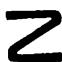
\includegraphics[keepaspectratio]{images/part002_69a966b6.jpg}}

注。A 为 Noether 环这一假设对于本推论是必要的。例如，设 A 是从 R 到自身的无穷可微映射组成的环，m 是 A 的由满足 \(f(0) = 0\) 的函数 f 组成的（极大）理想。立即可见，\(\bigcap_{n=0}^{\infty} m^{n}\) 是满足下述条件的函数 f 的集合：

\(f^{(n)}(0) = 0\) 对所有 \(n \geqslant 0\) 都成立；并且存在满足此条件而对所有 \(f(x) \neq 0\) 的 \(x \neq 0\) 都成立的函数，例如函数 \(f\)，它由 \(f(x) = e^{-1 / x^2}\)（\(x \neq 0\)）定义，且 \(f(0) = 0\)。

定义 1。设 A 为拓扑环。若 A 的一个双边理想 m 使得 A 上给定的拓扑是 m-进拓扑，则称 m 为 A 上该拓扑的定义理想。

设 A 为交换 Noether 环，m 为 A 的理想，t 为其根（第二章，第 2 节，第 6 号）。若 \(m'\) 是 m-进拓扑的定义理想，则存在整数 n \textgreater{} 0，使得 \(m'^{n} \subset m\)（第 2 节，第 5 号），因而 \(m' \subset t\)；反之，由于 A 是 Noether 环，存在整数 k \textgreater{} 0，使得 \(t^{k} \subset m\)（第二章，第 2 节，第 6 号，命题 15），因而 t 是 m-进拓扑的最大定义理想。

\subsection{Zariski 环}

命题 6。设 A 为交换 Noether 环，m 为 A 的理想。下列性质等价：

\begin{enumerate}
\def\labelenumi{(\alph{enumi})}
\item
  \(\mathfrak{m}\) 包含于 A 的 Jacobson 根。
\item
  每个有限生成的 A-模关于 m-进拓扑都是 Hausdorff 的。
\item
  对每个有限生成的 A-模 E，E 的每个子模关于 E 上的 m-进拓扑都是闭的。
\item
  A 的每个极大理想关于 m-进拓扑都是闭的。
\end{enumerate}

证明 (a) 蕴含 (b)。设 m 包含于 A 的 Jacobson 根，并令 E 为有限生成的 A-模。若 \(x \in E\) 和 \(m \in m\) 满足 \((1 - m)x = 0\)，则 x = 0，因为 1 - m 在 A 中可逆。于是由（第 2 号，命题 5），E 关于 m-进拓扑是 Hausdorff 的。

证明 (b) 蕴含 (c)。设 (b) 成立。令 E 为有限生成的 A-模，F 为 E 的子模。则 E/F 关于 m-进拓扑是 Hausdorff 的，而该拓扑正是 E 上 m-进拓扑的商拓扑；所以 F 在 E 中是闭的。

显然 (c) 蕴含 (d)。最后证明 (d) 蕴含 (a)。由 (d) 可知，对于 A 的每个极大理想 a，A/a 作为 A-模关于 m-进拓扑是 Hausdorff 的。这意味着 \(\mathfrak{m}(\mathrm{A}/\mathfrak{a}) \neq \mathrm{A}/\mathfrak{a}\)，除非 A/a 上的 m-进拓扑是最粗拓扑且 A/a 化为 0；但这是荒谬的，因为 A/a 是域。因此，m 在 A/a 中的典范像是 A/a 的一个不等于 A/a 的理想，故只能为 0；于是 \(m \subset a\)，这证明了 m 包含于 A 的 Jacobson 根。

定义 2。若拓扑环 A 是交换的、Noether 的，并且存在一个关于 A 上的拓扑的定义理想 m，满足命题 6 的等价条件，则称 A 为 Zariski 环。

Zariski 环 A 必然是 Hausdorff 的（命题 6），且其拓扑的每个定义理想都包含于 A 的 Jacobson 根。

\textbf{Zariski 环的例子}\par

\begin{enumerate}
\def\labelenumi{(\arabic{enumi})}
\item
  设 A 为交换 Noether 环，m 为 A 的理想。若 A 关于 m-进拓扑是 Hausdorff 且完备的，则根据第 2 节第 13 号引理 3，A 连同此拓扑是 Zariski 环。
\item
  Zariski 环的每个商环 A/b 都是 Zariski 环，因为它是 Noether 环，并且若 m 是 A 的定义理想，则 \(\mathfrak{m}(\mathbf{A}/\mathfrak{b}) = (\mathfrak{m} + \mathfrak{b})/\mathfrak{b}\) 包含于 A/b 的 Jacobson 根（代数，第八章，第 6 节，第 3 号，命题 7）。
\item
  设 A 为 Noether 半局部环，r 为其 Jacobson 根。则赋予 A r-进拓扑后，A 是 Zariski 环。当我们将 Noether 半局部环视为拓扑环时，所指的拓扑总是这一拓扑（另有说明时除外）。
\end{enumerate}

命题 7。设 A、A' 为两个交换环，h: A → A' 为环同态。假设 A 是 Noether 环，且 A' 是有限生成的 A-模（其结构由 h 定义）。设 m 为 A 的理想，m' = mA'。则：

\begin{enumerate}
\def\labelenumi{(\roman{enumi})}
\item
  对于 \(\mathfrak{m}'\)-进拓扑在 \(\mathbf{A}'\) 上为 Hausdorff，充要条件是 \(1 + h(\mathfrak{m})\) 中的元素都不是 \(\mathbf{A}'\) 中的零因子。
\item
  若赋予 A m-进拓扑后 A 是 Zariski 环，则赋予 A' m'-进拓扑后 A' 也是 Zariski 环。
\item
  若 \(h\) 是单射（从而将 \(\mathbf{A}\) 识别为 \(\mathbf{A}'\) 的子环），则 \(\mathfrak{m}'\)-进拓扑在 \(\mathbf{A}'\) 上诱导出在 \(\mathbf{A}\) 上的 \(\mathfrak{m}\)-进拓扑。
\end{enumerate}

回忆一下，A' 上的 m'-进滤过与 A'-这个 A-模上的 m-进滤过相同（第 2 节，第 1 号，例 3）。断言 (i) 因而是第 2 号命题 5 的特殊情形，断言 (iii) 是第 2 号定理 2 的特殊情形。最后证明 (ii)。设 A 连同 m-进拓扑是 Zariski 环，令 E' 为有限生成的 A'-模；它也是有限生成的 A-模，且 E' 上的 m-进滤过与 m'-进滤过相同；因此 E' 关于 m'-进拓扑是 Hausdorff 的。最后，A-模 A' 是 Noether 的，因而环 A' 是 Noether 的，这就完成了 A' 为 Zariski 环的证明。

\subsection{Noether 环的 Hausdorff 完备化}

设 A 为交换环，m 为 A 的理想，E 为 A-模；令 \(\hat{A}\) 和 \(\hat{E}\) 分别表示 A 和 E 关于 m-进拓扑的 Hausdorff 完备化，\(j_{E}\) 表示典范映射 \(E \rightarrow \hat{E}\)。A-双线性映射 \((a, x) \mapsto aj_{\mathrm{E}}(x)\) 从 \(\hat{A} \times E\) 到 \(\hat{E}\)，定义了一个 A-线性映射

\[
\alpha_ {\mathrm{E}} \colon \hat {\mathrm{A}} \otimes_ {\mathrm{A}} \mathrm{E} \rightarrow \hat {\mathrm{E}},
\]

称为典范映射。设 \(u: \mathrm{E} \to \mathrm{F}\) 是 A-模同态，\(\hat{u}\colon \hat{\mathbf{E}}\to \hat{\mathbf{F}}\) 是由取 Hausdorff 完备化得到的映射；对于 \(a\in \hat{\mathbf{A}},x\in \mathbf{E},\)

\[
\alpha_ {\mathrm{F}} (a \otimes u (x)) = a j _ {\mathrm{F}} (u (x)) = a \hat {u} (j _ {\mathrm{E}} (x)) = \hat {u} (\alpha_ {\mathrm{E}} (a \otimes x)),
\]

换言之，图

\pandocbounded{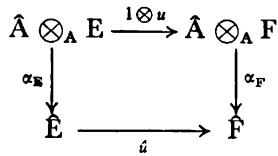
\includegraphics[keepaspectratio]{images/part002_24f0cc04.jpg}}

是交换的。最后，由第 2 节第 12 号命题 16 可知，若 E 有限生成，则同态 \(\alpha_{\mathbb{E}}\) 是满射。

定理 3。设 A 为交换 Noether 环，m 为 A 的理想，E、F、G 为三个有限生成的 A-模。则：

\begin{enumerate}
\def\labelenumi{(\roman{enumi})}
\item
  若 \(E \xrightarrow{u} F \xrightarrow{v} G\) 是 A-线性映射的正合列，则对 m-进拓扑取 Hausdorff 完备化所得的序列 \(\hat{E} \xrightarrow{\hat{u}} \hat{F} \xrightarrow{\hat{v}} \hat{G}\) 是正合的。
\item
  典范的 \(\hat{\mathbf{A}}\)-线性映射 \(\alpha_{\mathbf{E}}: \hat{\mathbf{A}} \otimes_{\mathbf{A}} \mathbf{E} \to \hat{\mathbf{E}}\) 是双射。
\item
  A-模 \(\hat{\mathbf{A}}\) 是平坦的。
\end{enumerate}

我们已经看到，u 和 v 是拓扑群的严格态射（第 2 号，定理 2 的推论）。断言 (i) 于是由第 2 节第 12 号引理 2 得出。当 E = A 时，断言 (ii) 显然成立；当 E 是有限生成自由 A-模时，立即可归约到此情形。一般地，E 有一个有限表示

\[
\mathrm{L} \xrightarrow {u} \mathrm{L} ^ {\prime} \xrightarrow {v} \mathrm{E} \longrightarrow 0
\]

（第一章，第 2 节，第 8 号，引理 8）。于是得到一个交换图

\pandocbounded{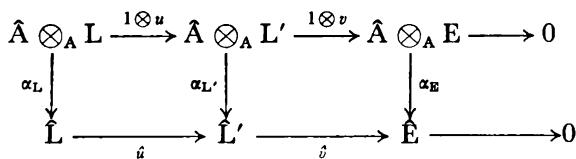
\includegraphics[keepaspectratio]{images/part002_14bc27b3.jpg}}

第一行是正合的（第一章，第 2 节，第 1 号，引理 1），由 (i) 第二行也正合。我们已经知道 \(\alpha_{\mathrm{E}}\) 是满射（第 2 节，第 12 号，命题 16）；另一方面，由于 \(\alpha_{\mathrm{L}}\) 和 \(\alpha_{\mathrm{L}'}\) 是双射且 \(1 \otimes v\) 是满射，根据第一章第 1 节第 4 号命题 2 的推论 2，\(\alpha_{\mathrm{E}}\) 是单射；这就证明了 (ii)。

由 (i) 和 (ii) 可知，若 \(a\) 是 \(A\) 的理想（必然有限生成），则典范映射 \(\hat{A} \otimes_{A} a \to \hat{A}\) 是单射，因为它是 \(\hat{a} \to \hat{A}\) 与 \(\alpha_{E}\) 的复合；这证明了 \(\hat{A}\) 是平坦的 A-模（第一章，第 2 节，第 3 号，命题 1）。

在定理 3 的条件下，\(\hat{\mathbf{A}}\otimes_{\mathbf{A}}\mathbf{E}\) 常识别为 \(\hat{\mathbf{E}}\)，借助典范映射 \(\alpha_{\mathbf{E}}\)。若 \(u\colon \mathbf{E}\to \mathbf{F}\) 是有限生成 A-模的同态，则由图（4）的交换性，\(\hat{u}\colon \hat{\mathbf{E}}\to \hat{\mathbf{F}}\) 识别为 \(1\otimes u\)。

推论 1。设 A 为交换 Noether 环，m 为 A 的理想，E 为有限生成的 A-模，F、G 为 E 的两个子模。赋予 A、E、F、G 以 m-进拓扑，令 i 为从 E 到 Ê 的典范映射。则：

\[
\begin{array}{r l} \hat {\mathbf {F}} = \hat {\mathbf {A}}. i (\mathbf {F}), & (\mathbf {F} + \mathbf {G}) ^ {\wedge} = \hat {\mathbf {F}} + \hat {\mathbf {G}}, \\ & (\mathbf {F} \cap \mathbf {G}) ^ {\wedge} = \hat {\mathbf {F}} \cap \hat {\mathbf {G}}, \\ & (\mathbf {F}: \mathbf {G}) ^ {\wedge} = \hat {\mathbf {F}}: \hat {\mathbf {G}}. \end{array}
\]

此外，若 a、b 是 A 的两个理想且 c = ab，则 \(\hat{c} = \hat{ab}\)。

根据定理 3，\(\hat{\mathbf{E}}\)、\(\hat{\mathbf{F}}\)、\(\hat{\mathbf{G}}\) 分别典范地识别为 \(\hat{\mathbf{A}} \otimes_{\mathbf{A}} \mathbf{E}\)、\(\hat{\mathbf{A}} \otimes_{\mathbf{A}} \mathbf{F}\)、\(\hat{\mathbf{A}} \otimes_{\mathbf{A}} \mathbf{G}\)，这就建立了前两个公式。第三个和第四个分别由第一章第 2 节第 6 号命题 6 及第 10 号命题 12 得出。最后，由于 \(\hat{\mathbf{a}} = \hat{\mathbf{A}}i(\mathfrak{a})\)、\(\hat{\mathfrak{b}} = \hat{\mathbf{A}}i(\mathfrak{b})\)、\(\hat{\mathfrak{c}} = \hat{\mathbf{A}}i(\mathfrak{c})\)，

\[
\hat {\mathfrak {c}} = \hat {\mathrm{A}} i (\mathfrak {a b}) = \hat {\mathrm{A}} i (\mathfrak {a}) i (\mathfrak {b}) = \hat {\mathfrak {a b}}.
\]

推论 2。设 A 为交换 Noether 环，m 为 A 的理想，\(\hat{\mathbf{A}}\) 为 A 关于 m-进拓扑的 Hausdorff 完备化。若元素 \(a \in \mathbf{A}\) 不是 A 中的零因子，则它的典范像 \(a'\) 在 \(\hat{\mathbf{A}}\) 中不是 \(\hat{\mathbf{A}}\) 中的零因子。

由于 \(\hat{\mathbf{A}}\) 是平坦的 A-模，该推论是第一章第 2 节第 4 号命题 3（i）的特殊情形。

推论 3。若 A 是交换 Noether 环，则形式幂级数环 A{[}{[}X₁, \ldots, Xₙ{]}{]} 是平坦的 A-模。

它是多项式环

\[
\mathbf {B} = \mathbf {A} [ \mathbf {X} _ {1}, \dots , \mathbf {X} _ {n} ]
\]

关于 m-进拓扑，其中 m 是不含常数项的多项式组成的集合（第 2 节，第 12 号，例 1）；由于 B 是 Noether 环（第 2 节，第 10 号，定理 2 的推论 2），根据定理 3，A{[}{[}X₁, \ldots, Xₙ{]}{]} 是平坦的 B-模；又由于 B 是自由 A-模，A{[}{[}X₁, \ldots, Xₙ{]}{]} 是平坦的 A-模（第一章，第 2 节，第 7 号，命题 8 的推论 3）。

命题 8。设 A 为交换 Noether 环，m 为 A 的理想，\(\hat{A}\) 为 A 关于 m-进拓扑的 Hausdorff 完备化，j 为从 A 到 \(\hat{A}\) 的典范映射。则：

\begin{enumerate}
\def\labelenumi{(\roman{enumi})}
\item
  \(\hat{\mathbf{A}}\) 是 Zariski 环，且 \(\hat{\mathfrak{m}} = \hat{\mathbf{A}}.j(\mathfrak{m})\) 是 \(\hat{\mathbf{A}}\) 的定义理想。
\item
  映射 \(\mathfrak{n} \mapsto \hat{\mathfrak{n}} = \hat{\mathbf{A}}.j(\mathfrak{n})\) 将 \(\mathbf{A}\) 中包含 \(\mathfrak{m}\) 的极大理想集双射到 \(\hat{\mathbf{A}}\) 的极大理想集，而 \(\mathfrak{q} \mapsto j^{-1}(\mathfrak{q})\) 是其逆双射。
\item
  设 \(\mathfrak{n}\) 是 \(\mathbf{A}\) 的包含 \(\mathfrak{m}\) 的极大理想。同态 \(j': \mathbf{A}_{\mathfrak{n}} \to \hat{\mathbf{A}}_{\hat{\mathfrak{n}}}\) 由 \(j\) 得到且是单射；若将 \(\mathbf{A}_{\mathfrak{n}}\) 通过 \(j\) 识别为 \(\hat{\mathbf{A}}_{\hat{\mathfrak{n}}}\) 的子环，则 \((\mathfrak{n}\mathbf{A}_{\mathfrak{n}})\)-进拓扑在 \(\mathbf{A}_{\mathfrak{n}}\) 上由 \(\hat{\mathfrak{n}}\)-进拓扑在 \(\hat{\mathbf{A}}_{\hat{\mathfrak{n}}}\) 上诱导，且 \(\mathbf{A}_{\mathfrak{n}}\) 在 \(\hat{\mathbf{A}}_{\hat{\mathfrak{n}}}\) 中关于 \(\hat{\mathfrak{n}}\)-进拓扑稠密。
\end{enumerate}

证明 (i)。由于 \(\mathfrak{m}\) 是有限生成的理想，\((\mathfrak{m}^n)^{\circ} = (\hat{\mathfrak{m}})^n = \mathfrak{m}^n\hat{\mathbf{A}}\)（第 2 节，第 12 号，命题 16 的推论 2），且 \(\hat{\mathbf{A}}\) 上的拓扑是 \(\hat{\mathfrak{m}}\)-进拓扑。由于 \(\hat{\mathbf{A}}/\hat{\mathfrak{m}}\) 同构于 \(\mathbf{A}/\mathfrak{m}\)，它是 Noether 环，而 \(\hat{\mathfrak{m}} = \mathfrak{m}\hat{\mathbf{A}}\) 是有限生成的 \(\hat{\mathbf{A}}\)-模，因而 \(\hat{\mathbf{A}}\) 是 Noether 环（第 2 节，第 10 号，定理 2 的推论 5）；最后，由于 \(\hat{\mathbf{A}}\) 关于 \(\hat{\mathfrak{m}}\)-进拓扑是 Hausdorff 且完备的，\(\hat{\mathbf{A}}\) 是 Zariski 环（第 3 号，例 1）。

断言 (ii) 立即由以下事实得出：由 j 得到的典范同态 \(A/m \rightarrow \hat{A}/\hat{m}\) 是双射，并且 \(\hat{A}\) 的每个极大理想都包含 \(\hat{m}\)，因为 \(\hat{A}\) 是 Zariski 环，故 \(\hat{A}\) 的 Jacobson 根包含 \(\hat{m}\)（第 3 号，命题 6）。

最后证明 (iii)。由于 \(\mathfrak{n} = j^{-1}(\hat{\mathfrak{n}}), j(\mathbf{A} - \mathfrak{n}) \subset \hat{\mathbf{A}} - \hat{\mathfrak{n}}\)，\(j\) 确实定义了同态 \(j' \colon \mathbf{A}_{\mathfrak{n}} \to \hat{\mathbf{A}}_{\hat{\mathfrak{n}}}\)（第二章，第 2 节，第 1 号，命题 2）。证明 \(j'\) 是单射；设 \(a \in \mathbf{A}, s \in \mathbf{A} - \mathfrak{n}\)，满足

\[
j ^ {\prime} (a / s) = j (a) / j (s) = 0;
\]

则存在 \(s' \in \hat{\mathbf{A}} - \hat{\mathfrak{n}}\)，使得 \(s'j(a) = 0\)（第二章，第 2 节，第 1 号，注 3），所以 \(j(a)\) 在 \(\hat{\mathbf{A}}\) 中的湮没子不包含于 \(\hat{\mathfrak{n}}\)。现在，若 \(\mathfrak{b}\) 是 \(a\) 在 \(\mathbf{A}\) 中的湮没子，则 \(j(a)\) 在 \(\hat{\mathbf{A}}\) 中的湮没子为 \(\mathfrak{b}\)（定理 3 的推论 1）；因而 \(\mathfrak{b} \not\subset \mathfrak{n}\)，这表明 \(a / s = 0\)。

此外，还有一个交换图

\[
\begin{array}{c} \mathrm{A} / \mathfrak {n} ^ {k} \longrightarrow \mathrm{A} _ {\mathfrak {n}} / (\mathfrak {n} \mathrm{A} _ {\mathfrak {n}}) ^ {k} \\ \stackrel {{h}} {{\downarrow}} \qquad \qquad \qquad \qquad \qquad \qquad \qquad \qquad \qquad \qquad \qquad \qquad \qquad \qquad \qquad \qquad \qquad \qquad \qquad \qquad \qquad \qquad \qquad \hat {\mathrm{A}} / \hat {\mathfrak {n}} ^ {k} \longrightarrow \hat {\mathrm{A}} _ {\hat {\mathfrak {n}}} / (\hat {\mathfrak {n}} \hat {\mathrm{A}} _ {\hat {\mathfrak {n}}}) ^ {k} \end{array}\tag{5}
\]

其中 \(h\) 和 \(h'\) 分别由 \(j\) 和 \(j'\) 得到，水平箭头是第二章第 3 节第 3 号命题 9 的典范同构。由于 \(n^k\) 是 A 的开理想（因为它包含 \(m^k\)），\(h\) 是双射，因而 \(h'\) 也是双射。这首先表明 \((\mathfrak{n}\mathbf{A}_{\mathfrak{n}})^k = j'((\hat{\mathfrak{n}}\hat{\mathbf{A}}_{\hat{\mathfrak{n}}})^k)\)，因而 \(\mathbf{A}_{\mathfrak{n}}\) 上的拓扑由 \(\hat{\mathbf{A}}_{\hat{\mathfrak{n}}}\) 上的拓扑诱导；此外，\(\hat{\mathbf{A}}_{\hat{\mathfrak{n}}} = \mathbf{A}_{\mathfrak{n}} + (\hat{\mathfrak{n}}\hat{\mathbf{A}}_{\hat{\mathfrak{n}}})^k\) 对所有 \(k > 0\) 都成立，因而 \(\mathbf{A}_{\mathfrak{n}}\) 在 \(\hat{\mathbf{A}}_{\hat{\mathfrak{n}}}\) 中处处稠密。

推论。设 A 为 Noether 局部环（分别为半局部环），m 为其 Jacobson 根。则 \(\hat{A}\) 是 Noether 局部环（分别为半局部环），其 Jacobson 根为 \(\hat{m}\)。

\(\hat{\mathbf{A}}\) 根据命题 8（i）是 Noether 环，其余结论由命题 8（ii）及定理 3 的推论 1 中的第三个公式得出。

\subsection{Zariski 环的完备化}

命题 9。设 A 为交换 Noether 环，m 为 A 的理想；赋予 A m-进拓扑。要使 \(\hat{\mathbf{A}}\) 成为忠实平坦的 A-模，充要条件是 A 为 Zariski 环。

对于每个有限生成的 A-模 M，典范映射 \(M \to M \otimes_{A} \hat{A}\) 可识别为从 M 到其关于 m-进拓扑的 Hausdorff 完备化的典范映射 \(M \to \hat{M}\)（第 4 号，定理 3），而该映射的核就是 M 中关于此拓扑的 \(\{0\}\) 的闭包。由于我们已经知道 \(\hat{A}\) 是平坦的 A-模（第 4 号，定理 3），命题由忠实平坦模的刻画（第一章，第 3 节，第 1 号，命题 1（b））和 Zariski 环的刻画（第 3 号，命题 6）得出。

若 A 是 Zariski 环且 E 是有限生成的 A-模，则根据命题 9，我们可以将 E 识别为 \(\hat{E}\) 的子集，借助典范映射 \(j_{E}: E \to \hat{E}\)。在此识别下：

推论 1。设 A 为 Zariski 环，E 为有限生成的 A-模，F 为 E 的子模。则 \(\mathbf{F} = \hat{\mathbf{F}} \cap \mathbf{E} = (\hat{\mathbf{A}}\mathbf{F}) \cap \mathbf{E}\)。

这是第一章第 3 节第 5 号命题 10（ii）的特殊情形，也可由第 3 号命题 6 得出。

推论 2。设 A 为 Zariski 环，E 为有限生成的 A-模。若 \(\hat{\mathbf{E}}\) 是自由的 \(\hat{\mathbf{A}}\)-模，则 E 是自由的 A-模。

设 \(\mathfrak{m}\) 为 \(\mathbf{A}\) 的定义理想，因而包含于 \(\mathbf{A}\) 的 Jacobson 根中。我们应用第二章第 3 节第 5 号命题 5 的判别法：典范映射 \(j_{\mathrm{E}}: \mathrm{E} \to \hat{\mathrm{E}}\) 定义了双射 \(i_{\mathrm{E}}: \mathrm{E} / \mathfrak{m}\mathrm{E} \to \hat{\mathrm{E}} / (\mathfrak{m}\mathrm{E})^{\wedge}\)；同样，典范映射 \(j_{\mathrm{A}}: \mathrm{A} \to \hat{\mathrm{A}}\) 定义了双射 \(i_{\mathrm{A}}: \mathrm{A} / \mathfrak{m} \to \hat{\mathrm{A}} / \hat{\mathfrak{m}}\)，它是环同构。于是 \((\mathfrak{m}\mathrm{E})^{\wedge} = \hat{\mathrm{A}}. \mathfrak{m}\mathrm{E} = \hat{\mathfrak{m}}\hat{\mathrm{E}}\)（第 4 号，定理 3），所以 \(\hat{\mathrm{E}} / (\mathfrak{m}\mathrm{E})^{\wedge}\) 具有一个 \((\hat{\mathrm{A}} / \hat{\mathfrak{m}})\)-模结构，并且（借助 \(i_{\mathrm{A}}\)）具有一个 \((\mathrm{A} / \mathfrak{m})\)-模结构。立即可见，\(i_{\mathrm{E}}\) 是 \((\mathrm{A} / \mathfrak{m})\)-线性的，因而是一个 \((\mathrm{A} / \mathfrak{m})\)-模同构。由于 \(\hat{\mathrm{E}} / \hat{\mathfrak{m}}\hat{\mathrm{E}}\) 是自由的 \((\hat{\mathrm{A}} / \hat{\mathfrak{m}})\)-模，\(\mathrm{E} / \mathfrak{m}\mathrm{E}\) 是自由的 \((\mathrm{A} / \mathfrak{m})\)-模。

另一方面，令 \(v: \mathfrak{m} \otimes_{\mathbf{A}} \mathbf{E} \to \mathbf{E}\) 为典范同态；由于 \((\mathfrak{m} \otimes_{\mathbf{A}} \mathbf{E}) \otimes_{\mathbf{A}} \hat{\mathbf{A}}\) 典范地识别为 \(\hat{\mathfrak{m}} \otimes_{\mathbf{A}} \hat{\mathbf{E}}\)，而 \(\mathbf{E} \otimes_{\mathbf{A}} \hat{\mathbf{A}}\) 识别为 \(\hat{\mathbf{E}}\)（第 4 号，定理 3），\(\hat{\mathbf{E}}\) 是自由的 \(\hat{\mathbf{A}}\)-模这一假设蕴含同态 \(v \otimes 1: \hat{\mathfrak{m}} \otimes_{\hat{\mathbf{A}}} \hat{\mathbf{E}} \to \hat{\mathbf{E}}\) 是单射。由于 \(\hat{\mathbf{A}}\) 是忠实平坦的 A-模（命题 9），我们得到 \(v\) 是单射（第一章，第 3 节，第 1 号，命题 2），因而上述判别法的应用条件确已满足。

推论 3。设 A 为 Zariski 环，且 \(\hat{\mathbf{A}}\) 是整环，\(\mathfrak{a}\) 是 A 的理想。若理想 \(\mathfrak{a}\hat{\mathbf{A}}\) 在 \(\hat{\mathbf{A}}\) 中是主理想，则 \(\mathfrak{a}\) 是主理想。这是推论 2 的特殊情形。

推论 4。设 A 为 Zariski 环，且 \(\hat{\mathbf{A}}\) 是整环，L 为 \(\hat{\mathbf{A}}\) 的分式域，\(\mathbf{K} \subset \mathbf{L}\) 为 A 的分式域；则 \(\hat{\mathbf{A}} \cap \mathbf{K} = \mathbf{A}\)。

显然 \(\mathbf{A} \subset \hat{\mathbf{A}} \cap \mathbf{K}\)；另一方面，若 \(x \in \hat{\mathbf{A}} \cap \mathbf{K}\)，则 \(\hat{\mathbf{A}}x \subset \hat{\mathbf{A}}\)，因而由于 \(\hat{\mathbf{A}}x = \hat{\mathbf{A}} \otimes_{\mathbf{A}} (\mathbf{A}x)\)（第 4 号，定理 3），有 \(\hat{\mathbf{A}} \otimes_{\mathbf{A}} ((\mathbf{A}x + \mathbf{A}) / \mathbf{A}) = 0\)。由于 \(\hat{\mathbf{A}}\) 是忠实平坦的 A-模（命题 9），我们得到 \(\mathbf{A}x \subset \mathbf{A}\)，所以 \(x \in \mathbf{A}\)。

推论 5。设 A 为交换 Noether 环，E、F 为两个有限生成的 A-模，u: E → F 为 A-同态。对于 A 的每个极大理想 m，令 A(m)（分别为 E(m)、F(m)）表示 A（分别为 E、F）关于 m-进拓扑的 Hausdorff 完备化，令 u(m): E(m) → F(m) 为 u 所对应的同态。u 为单射（分别为满射、双射、零映射）的充要条件是：对于 A 的每个极大理想 m，u(m) 都具有相应性质。

我们知道，要使 \(u\) 为单射（分别为满射、双射、零映射），充要条件是 \(u_{\mathfrak{m}}: \mathrm{E}_{\mathfrak{m}} \to \mathrm{F}_{\mathfrak{m}}\) 对每个极大理想 \(\mathfrak{m}\)（属于 \(\mathbf{A}\)）都具有相应性质（第二章，第 3 节，第 3 号，定理 1）。现在注意到，\(\mathbf{A}_{\mathfrak{m}}\) 是 Noether 局部环（第二章，第 2 节，第 4 号，命题 10 的推论 2），因而是 Zariski 环，并且存在典范的 A-代数同构 \(\hat{\mathbf{A}}_{\mathfrak{m}} \to \mathbf{A}(\mathfrak{m})\)（第 2 节，第 13 号，命题 18）。另一方面（第 4 号开头），存在交换图

\[
\begin{array}{l} \mathrm{E} _ {\mathfrak {m}} \otimes_ {\mathbf {A} _ {\mathfrak {m}}} \mathrm{A} (\mathfrak {m}) \longrightarrow \mathrm{E} \otimes_ {\mathbf {A}} \mathrm{A} (\mathfrak {m}) \longrightarrow \mathrm{E} (\mathfrak {m}) \\ u _ {\mathfrak {m}} \otimes 1 \Biggl \downarrow \qquad \qquad \qquad \qquad \Biggl \downarrow u \otimes 1 \qquad \qquad \Biggl \downarrow u (\mathfrak {m}) \\ \mathrm{F} _ {\mathfrak {m}} \otimes_ {\mathbf {A} _ {\mathfrak {m}}} \mathrm{A} (\mathfrak {m}) \longrightarrow \mathrm{F} \otimes_ {\mathbf {A}} \mathrm{A} (\mathfrak {m}) \longrightarrow \mathrm{F} (\mathfrak {m}) \end{array}
\]

左侧的水平箭头来自张量积的结合律以及同构 \(E_{m} \rightarrow E \otimes_{A} A_{m}\)、\(F_{m} \rightarrow F \otimes_{A} A_{m}\)；由于 E、F 是有限生成的 A-模，由第 4 号定理 3 可知该图的各行都是同构。因此问题归结为证明：\(u_{m}\) 是单射（分别为满射、双射、零映射）当且仅当 \(u_{m} \otimes 1\) 具有相应性质。但这是命题 9 所说的 \(\hat{A}_{m}\)（因而 \(A(m)\) 也）是忠实平坦的 \(A_{m}\)-模这一事实的结果（第一章，第 3 节，第 1 号，命题 1 和 2）。

命题 10。设 A、B 为两个 Zariski 环，\(\hat{A}\)、\(\hat{B}\) 为它们的完备化，\(f\colon A\to B\) 为连续环同态，\(\hat{f}\colon\hat{A}\to\hat{B}\) 为由 \(f\) 取完备化得到的同态；若 \(\hat{f}\) 是双射，则 B 是忠实平坦的 A-模。

由于 A、B 是 Hausdorff 的，\(\hat{f}\) 为双射这一假设首先蕴含 \(f\) 是单射。将 A（代数地）识别为 \(f(A)\)，这是借助 \(f\) 完成的；随后将 \(\hat{A}\) 识别为 \(\hat{B}\)，所对应的映射为 \(\hat{f}\)，于是得到包含关系 \(A \subset B \subset \hat{A} = \hat{B}\)；我们知道 \(\hat{A}\) 既是忠实平坦的 A-模，也是忠实平坦的 B-模（命题 9）；由此得到 B 是忠实平坦的 A-模（第一章，第 3 节，第 4 号，注 2）。

命题 11。设 A 为 Noether 局部环，m 为其极大理想，\(\hat{\mathbf{A}}\) 为其 m-进完备化，B 为满足 \(\mathbf{A} \subset \mathbf{B} \subset \hat{\mathbf{A}}\) 的环。假设 B 是 Noether 局部环，其极大理想 n 满足关系 \(n = mB\)。则

\[
\mathfrak {n} ^ {k} = \mathfrak {m} ^ {k} \mathrm{B} = \hat {\mathfrak {m}} ^ {k} \cap \mathrm{B}
\]

对所有 \(k \geqslant 1\)，\(\mathfrak{n}\)-进拓扑在 \(\mathbf{B}\) 上由 \(\hat{\mathfrak{m}}\)-进拓扑在 \(\hat{\mathbf{A}}\) 上诱导，\(\mathbf{B}\) 是忠实平坦的 \(\mathbf{A}\)-模，并且存在从 \(\hat{\mathbf{A}}\) 到 \(\mathfrak{n}\)-进完备化 \(\hat{\mathbf{B}}\) 的 \(\mathbf{B}\) 的同构，它延拓 \(\mathbf{A} \to \mathbf{B}\) 的典范单射。

只需验证关系 \(n^{k} = \hat{m}^{k} \cap B\)，因为 B 在 \(\hat{A}\) 中稠密，且 n-进拓扑由 \(\hat{m}\)-进拓扑诱导，所以最后一个断言由一般拓扑学第二章第 3 节第 9 号命题 18 的推论 1 得出，倒数第二个断言由命题 10 得出。单射 \(j_{A}: A \to \hat{A}\)（分别为 \(j_{B}: B \to \hat{A}\)）取商后定义了一个单同态

\[
i _ {\mathbf {A}} \colon \mathrm{A} / (\hat {\mathfrak {m}} \cap \mathrm{A}) \rightarrow \hat {\mathrm{A}} / \hat {\mathfrak {m}}
\]

（分别地，\(i_{B}\)：B/(m ∩ B) → Â/m）。我们知道 m ∩ A = m 且 \(i_{A}\) 是双射，因而 \(i_{B}\) 也是双射；这表明 B/(m ∩ B) 是域，所以 m ∩ B 是 B 的极大理想，从而 m ∩ B = n。~由于 \(\hat{A} = A + \hat{m}\)，\(B = A + n = A + mB\)；由 k 归纳可得

\[
\mathbf {B} = \mathbf {A} + \mathfrak {m} ^ {k} \mathbf {B} = \mathbf {A} + \mathfrak {n} ^ {k}
\]

对所有 \(k > 1\) 都成立。由于 \(\mathfrak{n}^k \subset \hat{\mathfrak{m}}^k \cap \mathbf{B}\)，只需证明 \(\hat{\mathfrak{m}}^k \cap \mathbf{B} \subset \mathfrak{n}^k\)；若 \(b \in \hat{\mathfrak{m}}^k \cap \mathbf{B}\)，可写成 \(b = a + z\)，其中 \(a \in \mathbf{A}\)、\(z \in \mathfrak{n}^k\)；于是

\[
a = b - z \in \hat {\mathfrak {m}} ^ {k} \cap \mathrm{A} = \mathfrak {m} ^ {k} \subset \mathfrak {n} ^ {k}
\]

且 \(b \in \mathfrak{n}^k\)。

* 此结果的一个重要应用情形如下：B 是完备赋值域上 n 个变量的整幂级数环，它们在 0 的邻域内收敛；A 是局部环

\[
\mathrm{K} [ \mathrm{X} _ {1}, \dots , \mathrm{X} _ {n} ] _ {\mathfrak {p}}
\]

其中 p 是由不含常数项的多项式组成的极大理想，\(\hat{A}\) 是形式幂级数环 \(K[[X_{1},\ldots,X_{n}]]\)。*

\pandocbounded{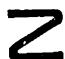
\includegraphics[keepaspectratio]{images/part002_72a4a9a7.jpg}}

注。满足 \(A \subset B \subset \hat{A}\)、其极大理想 n 等于 mB 且其 n-进拓扑由 \(\hat{A}\) 上的 m-进拓扑诱导的局部环 B 不一定是 Noether 环（习题 14）。

命题 12。设 A 为交换 Noether 环，m 为 A 的理想，S 为 A 的乘性子集 \(1 + m\)，E 为有限生成的 A-模。在这些条件下：

\begin{enumerate}
\def\labelenumi{(\roman{enumi})}
\item
  \(\mathbf{S}^{-1}\mathbf{A}\) 是 Zariski 环，且其拓扑为 \((\mathbf{S}^{-1}\mathfrak{m})\)-进拓扑。
\item
  典范映射 \(f \colon \mathbf{E} \to \mathbf{S}^{-1}\mathbf{E}\) 在 \(\mathbf{E}\) 赋予 \(\mathfrak{m}\)-进拓扑、\(\mathbf{S}^{-1}\mathbf{E}\) 赋予 \((\mathbf{S}^{-1}\mathfrak{m})\)-进拓扑时连续，且 \(\hat{f} \colon \hat{\mathbf{E}} \to (\mathbf{S}^{-1}\mathbf{E})^{\wedge}\) 是同构。
\end{enumerate}

\(1 + (\mathbf{S}^{-1}\mathfrak{m})\) 中的每个元素都具有如下形式：

\[
1 + (m / \left(1 + m ^ {\prime}\right)) = (1 + m + m ^ {\prime}) / (1 + m)
\]

其中 \(m \in m\) 且 \(m' \in m\)；所以它在 \(S^{-1}A\) 中可逆，这证明 \(S^{-1}m\) 包含于 \(S^{-1}A\) 的 Jacobson 根；由于 \(S^{-1}A\) 是 Noether 环（第二章，第 2 节，第 4 号，命题 10 的推论 2），\(S^{-1}A\) 连同 \((\mathrm{S}^{-1}\mathrm{m})\)-进拓扑是 Zariski 环，这证明了 (i)。证明 (ii)。对于所有 n \textgreater{} 0，

\[
\bar {f} ^ {- 1} ((S ^ {- 1} m) ^ {n} E) = \bar {f} ^ {- 1} (S ^ {- 1} (m ^ {n} E)) = m ^ {n} E:
\]

显然首先 \(f(\mathfrak{m}^n\mathrm{E}) \subset \mathrm{S}^{-1}\mathfrak{m}^n\mathrm{E}\)；反之，设 \(x\) 是 \(f^{-1}(\mathrm{S}^{-1}\mathfrak{m}^n\mathrm{E})\) 的一个元素；则存在 \(m', m''\) 属于 \(\mathfrak{m}\) 的元素以及 \(x'' \in \mathfrak{m}^n\mathrm{E}\)，使得 \((1 + m')((1 + m'')x - x'') = 0\)，从而 \((1 - m)x = x'\)，其中

\[
m = - \left(m ^ {\prime} + m ^ {\prime \prime} + m ^ {\prime} m ^ {\prime \prime}\right) \in \mathfrak {m}
\]

且 \(x' = (1 + m')x'' \in \mathfrak{m}^n\mathrm{E}\)；我们得到

\[
x = (1 + m + \dots + m ^ {n - 1}) x ^ {\prime} + m ^ {n} x \in \mathfrak {m} ^ {n} \mathrm{E}.
\]

这就证明了 \(f\) 是严格态射。此外，\(f\) 的核，即所有 \(x \in \mathbf{E}\) 满足存在某个 \(s \in \mathbf{S}\) 使得 \(sx = 0\) 的集合，与典范映射 \(j: \mathbf{E} \to \hat{\mathbf{E}}\) 的核相同（第 2 号，命题 5）。于是存在拓扑同构 \(f_0: j(\mathbf{E}) \to f(\mathbf{E})\)，使得 \(f = f_0 \circ j\)；由于 \(j\) 是拓扑同构，问题归结为验证 \(f(\mathbf{E})\) 在 \(\mathbf{S}^{-1}\mathbf{E}\) 中稠密。现在 \(\mathbf{S}^{-1}\mathbf{E}\) 的每个元素都可写成 \(x / (1 - m)\)，其中 \(m \in \mathfrak{m}\)，并且立即可验证

\[
x / (1 - m) \equiv ((1 + m + \dots + m ^ {n - 1}) x) / 1 (\mathrm{mod.} \mathrm{S} ^ {- 1} \mathrm{m} ^ {n} \mathrm{E})
\]

这就完成了证明。

\section{完备环中的提升}

\subsection{强互素多项式}

设 R 为交换环。若 R 的两个元素 x、y 的主理想 Rx、Ry 互素，则称 x、y 强互素，换言之（第二章，第 1 节，第 2 号），若 \(\mathbf{R}x + \mathbf{R}y = \mathbf{R}\)；这等价于存在两个元素 \(a, b\)（属于 \(\mathbf{R}\)），使得 \(ax + by = 1\)。

引理 1（“Euclid 引理”）。设 \(x, y\) 是 \(\mathbf{R}\) 中的两个强互素元素；若 \(z \in \mathbf{R}\) 满足 \(x\) 整除 \(yz\)，则 \(x\) 整除 \(z\)。

若 \(1 = ax + by\)，则 \(z = x(az) + (yz)b\)。

若 \(x\) 和 \(y\) 在 \(\mathbf{R}\) 中强互素，则

\[
\mathrm{R} x y = (\mathrm{R} x) \cap (\mathrm{R} y)
\]

（第二章，第 1 节，第 2 号，命题 5）；若 R 是整环，则两个强互素元素的最小公倍元等于它们的乘积（代数，第六章，第 1 节，第 8 号），因而按照代数第六章第 1 节第 12 号的意义它们互素。反之，若 R 是主理想整环，则两个互素元素也强互素，这由 Bézout 等式得出（代数，第七章，第 1 节，第 2 号，定理 1）。

对于多项式环，有如下结果：

命题 1。设 A 为交换环，P、P' 是 A{[}X{]} 中的两个强互素多项式。假设 P 是首一的，次数为 s。则 A{[}X{]} 中的每个多项式 T 都可以唯一写成如下形式：

\[
\mathrm{T} = \mathrm{PQ} + \mathrm{P} ^ {\prime} \mathrm{Q} ^ {\prime}\tag{1}
\]

其中 \(\mathbf{Q} \in \mathbf{A}[\mathbf{X}]\)、\(\mathbf{Q}' \in \mathbf{A}[\mathbf{X}]\)，且 \(\deg(\mathbf{Q}') < s\)。

若进一步有 \(\deg (\mathbf{T})\leqslant t\) 且 \(\deg (\mathbf{P}^{\prime})\leqslant t - s\)，则 \(\deg (\mathbf{Q})\leqslant t - s\)

由于 \(\mathbf{P}\) 是首一的，\(\mathrm{PR} \neq 0\) 对每个多项式 \(\mathbf{R} \neq 0\)（属于 \(\mathbf{A}[\mathbf{X}]\)）都成立，且此时 \(\deg(\mathrm{PR}) = s + \deg(\mathbf{R})\)。

设 \(\mathbf{T}\) 是 A{[}X{]} 中任意多项式。由于 P 和 \(\mathbf{P}'\) 生成的理想就是整个 A{[}X{]}，存在多项式 \(\mathbf{Q}_1\) 和 \(\mathbf{Q}_1'\)，使得

\[
\mathrm{T} = \mathrm{PQ} _ {1} + \mathrm{P} _ {1} ^ {\prime} \mathrm{Q} _ {1} ^ {\prime};
\]

由于 P 是次数为 s 的首一多项式，Euclid 除法（代数，第四章，第 1 节，第 5 号）表明存在两个多项式 Q'、Q'\,'，使得 Q'\_1 = PQ'\,' + Q'，其中 deg(Q') \textless{} s；于是得到

\[
\mathrm{T} = \mathrm{PQ} _ {1} + \mathrm{P} ^ {\prime} (\mathrm{PQ} ^ {\prime \prime} + \mathrm{Q} ^ {\prime}) = \mathrm{PQ} + \mathrm{P} ^ {\prime} \mathrm{Q} ^ {\prime}
\]

其中 \(Q = Q_{1} + P'Q''\)。为证明公式（1）的唯一性，只需证明关系式

\[
0 = \mathrm{PQ} + \mathrm{P} ^ {\prime} \mathrm{Q} ^ {\prime}, \quad \deg (\mathrm{Q} ^ {\prime}) <   s\tag{2}
\]

蕴含 \(Q = Q' = 0\)。现在，若（2）成立，则 \(P\) 整除 \(-PQ = P'Q'\)，又由于 \(P\) 和

\(P'\) 强互素，根据引理 1，\(P\) 整除 \(Q'\)；若 \(Q' \neq 0\)，则存在多项式 \(S \neq 0\)，使得 \(Q' = PS\)，从而

\[
\deg (\mathbf {Q} ^ {\prime}) = s + \deg (\mathbf {S}) \geqslant s,
\]

这就矛盾了。我们得到 \(Q' = 0\)，于是 PQ = 0，最后根据开头的注记得到 Q = 0。

最后，假设 \(\deg(T) \leqslant t\) 且 \(\deg(P') \leqslant t - s\)；将多项式 \(T\) 写成形式（1）后，

\[
\deg (\mathrm{P} ^ {\prime} \mathrm{Q} ^ {\prime}) \leqslant \deg (\mathrm{P} ^ {\prime}) + \deg (\mathrm{Q} ^ {\prime}) <   s + \deg (\mathrm{P} ^ {\prime}) \leqslant t
\]

因而

\[
s + \deg (Q) = \deg (P Q) = \deg (T - P ^ {\prime} Q ^ {\prime}) \leqslant t
\]

所以 \(\deg (\mathbb{Q})\leqslant t - s.\)

例。对于多项式 \(P \in A[X]\)，P 与 X - a 强互素（其中 \(a \in A\)）的充要条件是 \(P(a)\) 在 A 中可逆。因为若 P 与 X - a 强互素，则由命题 1，存在 \(c \in A\) 及多项式 \(Q \in A[X]\)，使得 \(cP + (X - a)Q = 1\)，从而 \(cP(a) = 1\)，且 \(P(a)\) 可逆。反之，由 Euclid 除法

\[
\mathbf {P} = (\mathbf {X} - a) \mathbf {R} + \mathbf {P} (a)
\]

并且，若 \(\mathrm{P}(a)=b^{-1}\)，其中 \(b\in A\)，则得到 \(1=b\mathrm{P}-b(\mathrm{X}-a)\mathrm{R}\)，这表明 P 与 X-a 强互素。

设 A、B 为两个交换环，\(f\colon\mathbf{A}\to\mathbf{B}\) 为环同态。若 \(\mathbf{P}=\sum_{i\geqslant0}a_{i}\mathbf{X}^{i}\) 是 \(\mathbf{A}[[\mathbf{X}]]\) 中的形式幂级数，令 \(\bar{f}(\mathbf{P})\) 表示形式幂级数 \(\sum_{i\geqslant0}f(a_{i})\mathbf{X}^{i}\)，它属于 \(\mathbf{B}[[\mathbf{X}]]\)。若 \(\mathbf{P}\) 是多项式，则 \(\bar{f}(\mathbf{P})\) 也是多项式；若进一步 \(\mathbf{P}\) 是首一的，则 \(\bar{f}(\mathbf{P})\) 也是首一的，且次数与 \(\mathbf{P}\) 相同。最后，\(\mathbf{P}\mapsto\bar{f}(\mathbf{P})\) 显然是从 \(\mathbf{A}[[\mathbf{X}]]\) 到 \(\mathbf{B}[[\mathbf{X}]]\) 的同态，它延拓 \(f\)，并将 \(\mathbf{X}\) 映到 \(\mathbf{X}\)。在本段其余部分中，我们将始终以此意义使用记号 \(\bar{f}\)。

命题 2。设 A、B 为两个交换环，f 为从 A 到 B 的同态，P、P' 为 A{[}X{]} 中的两个多项式。若 P 与 P' 在 A{[}X{]} 中强互素，则 \(\bar{f}(\mathbf{P})\) 与 \(\bar{f}(\mathbf{P}')\) 在 B{[}X{]} 中强互素。反之，若 \(f\) 是满射，且其核包含于 A 的 Jacobson 根中，并且 P 是首一的，则结论也成立。

假设 P 与 \(P'\) 强互素；则存在多项式 Q、\(Q'\)，属于 A{[}X{]}，使得 \(PQ + P'Q' = 1\)；从而得到

\[
\bar {f} (\mathbf {P}) \bar {f} (\mathbf {Q}) + \bar {f} (\mathbf {P} ^ {\prime}) \bar {f} (\mathbf {Q} ^ {\prime}) = 1,
\]

由此得到第一个断言。为证明第二个断言，令 a 表示 f 的核；

令 \(\mathbf{E} = \mathbf{A}[\mathbf{X}]\)，令 \(\mathbf{F}\) 为 \(\mathbf{E}\) 中由 \(\mathbf{P}\) 和 \(\mathbf{P}'\) 生成的理想；由于 \(f\) 是满射且 \(\bar{f}(\mathbf{P})\) 首一，命题 1 表明，对于每个多项式 \(\mathbf{T} \in \mathbf{A}[\mathbf{X}]\)，存在两个多项式 \(\mathbf{Q}, \mathbf{Q}'\)，属于 \(\mathbf{A}[\mathbf{X}]\)，使得

\[
\bar {f} (\mathrm{T}) = \bar {f} (\mathrm{P}) \bar {f} (\mathrm{Q}) + \bar {f} (\mathrm{P} ^ {\prime}) \bar {f} (\mathrm{Q} ^ {\prime}),
\]

于是有关系 \(E = F + aE\)。现在，E/F 是有限生成的 A-模，因为每个多项式模 P 同余于一个次数 \(<\deg(P)\) 的多项式，而 P 是首一的。由于 \(E/F = a(E/F)\)，且 a 包含于 A 的 Jacobson 根中，Nakayama 引理表明 \(E/F = 0\)（代数，第八章，第 6 节，第 3 号，命题 6 的推论 2），这意味着 P 与 \(P'\) 强互素。

\subsection{限制形式幂级数}

定义 1。若交换拓扑环 A 存在一个由 A 的理想组成的 0 的邻域基本系 B，则称 A 具有线性拓扑（并称其拓扑是线性的）。

注意，在这样的环中，\(\mathfrak{S} \in \mathcal{B}\) 中的理想是开且闭的（一般拓扑学，第三章，第 2 节，第 1 号，命题 4 的推论）。对于所有 \(\mathfrak{S} \in \mathcal{B}\)，商拓扑环 A/\(\mathfrak{S}\) 是离散的；对于 \(\mathfrak{S} \in \mathcal{B}\)、\(\mathfrak{S}' \in \mathcal{B}\)、\(\mathfrak{S}' \subset \mathfrak{S}\)，令

\[
h _ {\mathfrak {S S} ^ {\prime}} \colon \mathrm{A} / \mathfrak {S} ^ {\prime} \rightarrow \mathrm{A} / \mathfrak {S}
\]

是典范映射。我们知道（一般拓扑学，第三章，第 7 节，第 3 号），\((\mathbf{A} / \mathfrak{S}, h_{\mathfrak{S}\mathfrak{S}'})\) 是离散环的逆系统（指标集为 \(\mathcal{B}\)，按 \(\supset\) 排序且有向），其逆极限是完备的 Hausdorff 线性拓扑环 \(\tilde{\mathbf{A}}\)；此外（同上，命题 2），定义了严格态射 \(i: \mathbf{A} \to \tilde{\mathbf{A}}\)，其核是 \(\{0\}\) 在 \(\mathbf{A}\) 中的闭包，像在 \(\tilde{\mathbf{A}}\) 中处处稠密，因此 \(\tilde{\mathbf{A}}\) 典范地识别为 \(\mathbf{A}\) 的 Hausdorff 完备化。

定义 2。给定交换拓扑环 A，形式幂级数

\[
\mathbf {T} = \sum_ {(n _ {i})} c _ {n _ {1} n _ {2} \dots n _ {p}} \mathbf {X} _ {1} ^ {n _ {1}} \mathbf {X} _ {2} ^ {n _ {2}} \dots \mathbf {X} _ {p} ^ {n _ {p}}
\]

若属于环 \(\mathbf{A}[[\mathbf{X}_1,\ldots ,\mathbf{X}_p]]\)，并且对于 A 中 0 的每个邻域 \(\mathbf{V}\)，系数 \(c_{n_1n_2\dots n_p}\) 中不属于 \(\mathbf{V}\) 的只有有限多个，则称其为限制的（换言之，族 \((c_{n_1n_2\dots n_p})\) 关于 \(\mathbf{N}^p\) 的有限子集补集滤子在 A 中趋于 0）。

若 A 具有线性拓扑，则 \(A[[X_{1},\ldots,X_{p}]]\) 中的限制形式幂级数构成 \(A[[X_{1},\ldots,X_{p}]]\) 的子环，记为 \(A\{X_{1},\ldots,X_{p}\}\)：因为若 \(T=\sum_{(n_{i})}c_{n_{1}\ldots n_{p}}X_{1}^{n_{1}}\ldots X_{p}^{n_{p}}\)、\(T'=\sum_{(n_{i})}c_{n_{1}\ldots n_{p}}^{'}X_{1}^{n_{1}}\ldots X_{p}^{n_{p}}\) 是两个限制形式幂级数，且 \(\mathfrak{S}\) 是 A 中 0 的一个邻域并且是 A 的理想，则存在整数 \(m\)，使得 \(c_{n_1\ldots n_p} \in \mathfrak{S}\) 且 \(c_{n_1\ldots n_p}' \in \mathfrak{S}\) 对每个指标组 \((n_1, \ldots, n_p)\) 都成立，只要至少有一个 \(n_k \geqslant m\)，其中 \(k\) 为指标；现在，若

\[
\mathrm{T} ^ {\prime \prime} = \mathrm{TT} ^ {\prime} = \sum_ {(n _ {i})} c _ {n _ {1} \dots n _ {p}} ^ {\prime \prime} \mathrm{X} _ {1} ^ {n _ {1}} \dots \mathrm{X} _ {p} ^ {n _ {p}},
\]

于是 \(c_{n_1 \ldots n_p}'' = \sum c_{r_1 \ldots r_p} c_{s_1 \ldots s_p}'\)，其中指标组 \((r_k), (s_k)\) 满足 \(r_k + s_k = n_k\)（\(1 \leqslant k \leqslant p\)）。我们得到，若 \(n_k \geqslant 2m\)，则 \(r_k \geqslant m\) 或 \(s_k \geqslant m\)，因而由于 \(\mathfrak{S}\) 是理想，有 \(c_{n_1 \ldots n_p}'' \in \mathfrak{S}\)，只要 \(n_k \geqslant 2m\) 对至少一个 \(k\) 成立，这就证明了我们的断言。此外，限制形式幂级数的每个导数 \(\partial T / \partial X_i\)（\(1 \leqslant i \leqslant p\)）都是限制的，这立即由定义以及邻域 \(\mathfrak{S} \in \mathcal{B}\) 是 A 的加法子群这一事实得出。

若 A 是离散的，则限制形式幂级数环就是多项式环 \(A[X_{1},\ldots,X_{p}]\)。

以下始终假设 A 具有线性拓扑，并令 \(\mathcal{B}\) 为 A 中由 A 的理想组成的 0 的邻域基本系；对于所有 \(\mathfrak{S} \in \mathcal{B}\)，令 \(p_{\mathfrak{S}}: A \to A/\mathfrak{S}\) 为典范同态。根据定义，对于每个限制形式幂级数 \(T \in A\{X_{1}, \ldots, X_{p}\}\)，

\[
\bar {p} _ {\Im} (\mathrm{T}) \in (\mathrm{A} / \Im) [ \mathrm{X} _ {1}, \dots , \mathrm{X} _ {p} ].
\]

显然

\[
((\mathbf {A} / \mathfrak {S}) [ \mathbf {X _ {1}}, \dots , \mathbf {X _ {p}} ], \bar {h} _ {\mathfrak {S} \mathfrak {S} ^ {\prime}})
\]

是环的逆系统（相对于有向指标集 \(\mathcal{B}\)），而 \((\bar{p}_{3})\) 是同态的逆系统 \(\mathrm{A}\{\mathrm{X}_1,\dots ,\mathrm{X}_p\} \to (\mathrm{A} / \Im)[\mathrm{X}_1,\dots ,\mathrm{X}_p]\)；由于每个多项式都是限制形式幂级数，\(\bar{p}_{3}\) 是满射；其核 \(\mathrm{N}_{3}\) 是 \(\mathrm{A}\{\mathrm{X}_1,\dots ,\mathrm{X}_p\}\) 的理想，由所有系数都属于 \(\Im\) 的限制形式幂级数组成；赋予 \(\mathrm{A}\{\mathrm{X}_1,\dots ,\mathrm{X}_p\}\) 以（线性）拓扑，使 \(\mathrm{N}_{3}\)（其中 \(\Im \in \mathcal{B}\)）构成 0 的邻域基本系（这个拓扑显然只取决于 A 上的拓扑）。于是由一般拓扑学第三章第 7 节第 3 号命题 2 可知

\[
\pi = \varprojlim_ {\mathfrak {S}} \bar {p} _ {\mathfrak {S}}: \mathrm{A} \{\mathrm{X} _ {1}, \dots , \mathrm{X} _ {p} \} \rightarrow \varprojlim_ {\mathfrak {S}} (\mathrm{A} / \mathfrak {S}) [ \mathrm{X} _ {1}, \dots , \mathrm{X} _ {p} ]\tag{3}
\]

是严格态射，其核是 \(\{0\}\) 在 \(\mathbf{A}\{\mathbf{X}_1,\ldots ,\mathbf{X}_p\}\) 中的闭包，且其像在

\[
\mathrm{A} ^ {\prime} = \lim _ {\leftarrow \mathfrak {S}} (\mathrm{A} / \mathfrak {S}) [ \mathrm{X} _ {1}, \dots , \mathrm{X} _ {p} ].
\]

命题 3。若具有线性拓扑的交换环 A 是 Hausdorff 且完备的，则典范同态 \(\pi\) 是拓扑环同构。

对所有 \((n_1, \ldots, n_p) \in \mathbf{N}^p\) 以及所有 \(\mathfrak{S} \in \mathcal{B}\)，令 \(\phi_{n_1 \ldots n_p}^{\mathfrak{S}}\) 为映射 \((\mathrm{A} / \mathfrak{S})[\mathrm{X}_1, \ldots, \mathrm{X}_p] \to \mathrm{A} / \mathfrak{S}\)，它将每个多项式映到该多项式中 \(\mathrm{X}_1^{n_1} \ldots \mathrm{X}_p^{n_p}\) 的系数；显然，\(\phi_{n_1 \ldots n_p}^{\mathfrak{S}}\) 构成 \((\mathrm{A} / \mathfrak{S})\)-模同态的逆系统（相对于有序集 \(\mathcal{B}\)），并且根据假设，\(\mathbf{A}\) 典范地识别为 \(\varprojlim_{\mathfrak{S}} (\mathrm{A} / \mathfrak{S})\)，所以 \(\phi_{n_1 \ldots n_p} = \varprojlim_{\mathfrak{S}} \phi_{n_1 \ldots n_p}^{\mathfrak{S}}\) 是从 \(\mathrm{A}'\) 到 \(\mathbf{A}\) 的连续 A-同态。对于每个元素 \(S = (S_{\mathfrak{S}})_{\mathfrak{S} \in \mathcal{B}}\)，属于 \(\mathrm{A}'\)，我们将看到，形式幂级数 \(T = \sum_{(n_i)} \phi_{n_1 \ldots n_p}(S) X_1^{n_1} \ldots X_p^{n_p}\) 是限制的，并满足 \(\pi(T) = S\)。对于所有 \(\mathfrak{S} \in \mathcal{B}\) 以及所有 \(\mathfrak{S}' \in \mathcal{B}\) 满足 \(\mathfrak{S}' \subset \mathfrak{S}\)，若关系 \(\phi_{n_1 \ldots n_p}^{\mathfrak{S}}(S_{\mathfrak{S}}) = 0\)，则

\[
\phi_ {n _ {1} \dots n _ {p}} ^ {\mathfrak {S} ^ {\prime}} (\mathrm{S} _ {\mathfrak {S} ^ {\prime}}) \in \mathfrak {S} / \mathfrak {S} ^ {\prime};
\]

由于 \(S_{\mathfrak{S}}\) 是多项式，我们看到，\(\phi_{n_{1}\ldots n_{p}}(S) \in \mathfrak{S}\)，除了有限多个 \((n_{1}, \ldots, n_{p})\) 之外；这些有限多个指标组满足 \(\phi_{n_{1}\ldots n_{p}}^{\mathfrak{S}}(S_{\mathfrak{S}}) \neq 0\)。这证明了第一个断言；第二个断言由定义得出。由于 A 是 Hausdorff 的，\(N_{\mathfrak{S}}\) 的交化为 0，因而 \(\pi\) 是双射；由于 \(\pi\) 是严格态射，这就完成了证明。

命题 4。设 A、B 为两个具有线性拓扑的交换环，B 是 Hausdorff 且完备的，\(u: \mathbf{A} \to \mathbf{B}\) 是连续同态。对于 B 中的每个元素族 \(\mathbf{b} = (b_i)_{1 \leq i \leq p}\)，存在唯一的连续同态

\[
\tilde {u} \colon \mathrm{A} \{\mathrm{X} _ {1}, \dots , \mathrm{X} _ {p} \} \rightarrow \mathrm{B}
\]

使得 \(\tilde{u}(a) = u(a)\) 对所有 \(a \in \mathbf{A}\) 都成立，并且 \(\tilde{u}(\mathbf{X}_i) = b_i\) 对 \(1 \leqslant i \leqslant p\) 都成立。

存在唯一同态 \(v \colon A[X_1, \ldots, X_p] \to B\)，使得 \(v(a) = u(a)\) 对 \(a \in A\) 都成立，并且 \(v(X_i) = b_i\) 对 \(1 \leqslant i \leqslant p\) 都成立。此外，若 \(\mathfrak{H}\) 是 \(B\) 中的一个 0 的邻域且为理想，则 \(\bar{u}^{-1}(\mathfrak{H}) = \mathfrak{I}\) 是 \(A\) 的一个理想且为 0 的邻域，并且对于每个多项式 \(P \in N_{\mathfrak{S}}\)，显然 \(v(P) \in \mathfrak{H}\)，所以 \(v\) 连续。由于 \(A[X_1, \ldots, X_p]\) 在 \(A\{X_1, \ldots, X_p\}\) 中稠密，\(\tilde{u}\) 的存在性和唯一性由一般拓扑学第三章第 3 节第 3 号命题 5 以及恒等式延拓原理得出。

在 \(\mathbf{A} = \mathbf{B}\) 且 \(u\) 为恒等映射的特殊情形，我们把 \(f(b_{1},\ldots ,b_{p})\) 或 \(f(\mathbf{b})\) 作为 \(\tilde{u} (f)\) 的值，其中 \(f\in \mathrm{A}\{\mathbf{X}_1,\dots ,\mathbf{X}_p\}\)。

\textbf{注}\par

\begin{enumerate}
\def\labelenumi{(\arabic{enumi})}
\item
  命题 4 证明了：对于一个假定为 Hausdorff 且完备的环 A 中的每个闭理想 \(\mathfrak{a}\)，关系 \(b_{i} \in \mathfrak{a}\) 对 \(1 \leqslant i \leqslant p\) 成立时，都有 \(f(b_{1}, \ldots, b_{p}) \in \mathfrak{a}\)，其中每个限制形式幂级数 \(f \in \mathrm{A}\{\mathrm{X}_{1}, \ldots, \mathrm{X}_{p}\}\) 均可取。
\item
  设 \(\mathbf{A}\) 具有线性拓扑；令 \(r\) 为满足
\end{enumerate}

\(1 \leqslant r \leqslant p\) 的整数，并赋予环 \(\mathrm{A}\{\mathrm{X}_1, \ldots, \mathrm{X}_r\}\) 以上述拓扑。则拓扑环 \(\mathrm{A}\{\mathrm{X}_1, \ldots, \mathrm{X}_p\}\) 可识别为限制形式幂级数环

\[
(\mathrm{A} \{\mathrm{X} _ {1}, \dots , \mathrm{X} _ {r} \}) \{\mathrm{X} _ {r + 1}, \dots , \mathrm{X} _ {p} \}
\]

这立即由定义得出。

\begin{enumerate}
\def\labelenumi{(\arabic{enumi})}
\setcounter{enumi}{2}
\tightlist
\item
  采用注 2 的记号，再假设 A 是 Hausdorff 且完备的，并将每个限制形式幂级数 \(f \in \mathrm{A}\{\mathbf{X}_1, \ldots, \mathbf{X}_p\}\) 写成如下形式：
\end{enumerate}

\[
f = \sum_ {(n _ {i})} c _ {n _ {r + 1} \dots n _ {p}} (\mathrm{X} _ {1}, \dots , \mathrm{X} _ {r}) \mathrm{X} _ {r + 1} ^ {n _ {r + 1}} \dots \mathrm{X} _ {p} ^ {n _ {p}}
\]

其中 \(c_{n_{r+1}\ldots n_p}\) 是限制形式幂级数。对于 A 中元素组成的每个组 \(\mathbf{x} = (x_1, \ldots, x_r)\)，令

\[
b _ {n _ {r + 1} \dots n _ {p}} = c _ {n _ {r + 1} \dots n _ {p}} (x _ {1}, \dots , x _ {p}).
\]

由注 1 立即可见，\(\sum_{(n_i)} b_{n_r+1 \ldots n_p} X_{r+1}^{n_r+1} \ldots X_p^{n_p}\) 是限制形式幂级数，记为 \(f(x_1, \ldots, x_r, X_{r+1}, \ldots, X_p)\)；称其为用 \(x_i\) 代替 \(X_i\)（对 \(1 \leqslant i \leqslant r\)）于形式幂级数 \(f\) 中所得到的级数。

\subsection{Hensel 引理}

在拓扑环 A 中，若元素 x 满足 0 是序列 \((x^{n})_{n\geqslant0}\) 的极限，则称 x 是拓扑幂零的。若 A 是具有线性拓扑的交换环，则称 x 拓扑幂零，是指对于 A 的每个开理想 \(\mathfrak{S}\)，x 在 A/\(\mathfrak{S}\) 中的典范像是该环的幂零元。若 \(r_{\mathfrak{S}}\) 是 A/\(\mathfrak{S}\) 的幂零根，则显然 \((r_{\mathfrak{S}})\) 是子集的逆系统，而 A 的拓扑幂零元集 t 是 \(r=\lim_{\leftarrow \mathfrak{S}}r_{\mathfrak{S}}\) 在

典范同态 \(\mathbf{A} \to \lim_{\leftarrow \mathfrak{S}} \mathbf{A} / \mathfrak{S}\) 下的逆像；因此它是 \(\mathbf{A}\) 的闭理想。若进一步 \(\mathbf{A}\) 是 Hausdorff 且完备的，则此理想包含于 \(\mathbf{A}\) 的 Jacobson 根中，并且元素 \(x \in \mathbf{A}\) 可逆的充要条件是其模 \(t\) 的类在 \(\mathbf{A} / t\) 中可逆（第 2 节，第 13 号，引理 3）。

注意，若 A 是环且 m 是 A 的双边理想，则 m 中的元素关于 m-进拓扑都是拓扑幂零的。

定理 1（Hensel）。设 A 为完备的 Hausdorff 线性拓扑交换环。设 m 是 A 的闭理想，其元素都是拓扑幂零的。令 B = A/m 为商拓扑环，\(\varphi: A \to B\) 为典范映射。令 R 为 A\{X\} 中的限制形式幂级数，\(\overline{\mathrm{P}}\) 为 B{[}X{]} 中的首一多项式，\(\overline{\mathrm{Q}}\) 为 B\{X\} 中的限制形式幂级数。假设 \(\overline{\varphi}(\mathrm{R}) = \overline{\mathrm{P}}\) 。\(\overline{\mathrm{Q}}\)，并且 \(\overline{\mathrm{P}}\) 与 \(\overline{\mathrm{Q}}\) 在 B\{X\} 中强互素。则存在唯一的有序对 (P, Q)，其中 \(\mathbf{P} \in \mathbf{A}[\mathbf{X}]\) 是首一多项式，\(\mathbf{Q} \in \mathbf{A}\{\mathbf{X}\}\) 是限制形式幂级数，并满足

\[
\mathrm{R} = \mathrm{P}. \mathrm{Q}, \quad \overline {{{\varphi}}} (\mathrm{P}) = \overline {{{\mathrm{P}}}}, \quad \overline {{{\varphi}}} (\mathrm{Q}) = \overline {{{\mathrm{Q}}}}.\tag{4}
\]

此外，P 与 Q 在 A\{X\} 中强互素；若 R 是多项式，则 Q 也是多项式。

证明分为四步。在前三步中假设 A 是离散的，此时 R 和 \(\overline{Q}\) 是多项式。

\textbf{(1) \(\mathfrak{m}^2 = 0\)}\par

设 S、T 是 A{[}X{]} 中的两个多项式，S 是首一的，且 \(\overline{\varphi}(S) = \overline{P}\)、\(\overline{\varphi}(T) = \overline{Q}\)；第 1 号命题 2 表明 S、T 强互素；所以（第 1 号，命题 1）存在唯一的 A{[}X{]} 中的多项式有序对 (S', T')，使得

\[
\mathrm{R} - \mathrm{ST} = \mathrm{ST} ^ {\prime} + \mathrm{TS} ^ {\prime} \quad \text { and } \quad \deg (\mathrm{S} ^ {\prime}) <   \deg (\mathrm{S}) = \deg (\overline {{\mathrm{P}}}).\tag{5}
\]

多项式 \(P = S + TS'\)、\(Q = T + T'\) 就是问题的解；事实上

\[
\overline {{{\mathbf {P}}}} \cdot \overline {{{\varphi}}} (\mathbf {T} ^ {\prime}) + \overline {{{\mathbf {Q}}}} \cdot \overline {{{\varphi}}} (\mathbf {S} ^ {\prime}) = \overline {{{\varphi}}} (\mathbf {S T} ^ {\prime} + \mathbf {T S} ^ {\prime}) = \overline {{{\varphi}}} (\mathbf {R} - \mathbf {S T}) = 0.\tag{6}
\]

由于 \(\overline{\mathbf{P}}\) 是首一的，\(\overline{\mathbf{P}}\) 与 \(\overline{\mathbf{Q}}\) 强互素，且

\[
\deg (\overline {{{\varphi}}} (S ^ {\prime})) <   \deg (\overline {{{\mathbf {P}}}}),
\]

第 1 号命题 1 表明 \(\bar{\varphi}(\mathbf{S}') = \bar{\varphi}(\mathbf{T}') = 0\)，换言之，\(\mathbf{S}'\) 和 \(\mathbf{T}'\) 的系数属于 \(\mathfrak{m}\)，而关系 \(\mathfrak{m}^2 = 0\) 给出

\[
\mathrm{PQ} = \mathrm{ST} + \mathrm{ST} ^ {\prime} + \mathrm{TS} ^ {\prime} = \mathrm{R},
\]

这满足关系（4）。由于 \(\overline{\varphi}(\mathbf{P}) = \overline{\mathbf{P}}\) 且 \(\overline{\varphi}(\mathbf{Q}) = \overline{\mathbf{Q}}\)，\(\mathbf{P}\) 与 \(\mathbf{Q}\) 强互素（第 1 号，命题 2）；最后，若 \(\mathbf{P}_1\) 和 \(\mathbf{Q}_1\) 是 A{[}X{]} 中满足（4）的另外两个多项式，且 \(\mathbf{P}_1\) 是首一的，则必有 \(S_1' = P_1 - S\)、\(T_1' = Q_1 - T\)、\(\deg(S_1') < \deg(S)\) 以及 \(R - ST = ST_1' + TS_1'\)，因为 \(S_1'\) 和 \(T_1'\) 的系数属于 \(m\)；但命题 1 随即证明 \(S' = S_1'\) 且 \(T' = T_1'\)，这就证明了有序对 \((P, Q)\) 的唯一性。

\textbf{(2) \(\mathfrak{m}\) 是幂零的}\par

令 \(n\) 为满足 \(m^n = 0\) 的最小整数，并对 \(n > 2\) 作归纳论证；定理在 \(n = 2\) 时已经证明。令 \(A' = A / m^{n-1}\)、\(m' = m / m^{n-1}\)；由于 \(m'^{n-1} = 0\)，存在唯一的有序对 \((P', Q')\)，其元素是 \(A'[X]\) 中的多项式，使得 \(P'\) 是首一的，\(R' = P'Q'\)，\(\bar{\psi}(P') = \overline{P}\) 且 \(\bar{\psi}(Q') = \overline{Q}\)，其中 \(\psi\) 表示典范同态 \(A' \to A'/m' = B\)，\(\theta\) 表示典范同态 \(A \to A'\)，且 \(R' = \bar{\theta}(R)\)。另一方面，由于 \((\mathfrak{m}^{n-1})^{2}=0\)，存在唯一的有序对 \((\mathrm{P},\mathrm{Q})\)，其元素是 A{[}X{]} 中的多项式，使得 P 是首一的且 \(R=PQ,\bar{\theta}(P)=\overline{P},\bar{\theta}(Q)=\overline{Q}\)；由于 \(\phi=\psi\circ\theta\)，这表明满足（4）的 P、Q 存在且唯一；此外，根据归纳假设，\(P'\) 与 \(Q'\) 强互素，因而 P 与 Q 也强互素。

\textbf{(3) A 是离散的}\par

注意，在此情形 m 不再必然是幂零的，但根据假设它总是幂理想。设 \(P_{0}\)、\(Q_{0}\) 是 A{[}X{]} 中的两个多项式，满足 \(\overline{\varphi}(P_{0}) = \overline{P}\)、\(\overline{\varphi}(Q_{0}) = \overline{Q}\)，且 \(P_{0}\) 是首一的。考虑 A 中由 \(R - P_{0}Q_{0}\) 的系数生成的理想 n；它是有限生成的且包含于 m，因而是幂零的（第二章，第 2 节，第 6 号，命题 15）；按定义，若 \(\psi: A \to A/n\) 是典范映射，则 \(\overline{\psi}(R) = \overline{\psi}(P_{0})\overline{\psi}(Q_{0})\)。此外，\(\overline{\psi}(P_{0})\) 与 \(\overline{\psi}(Q_{0})\) 强互素；这是由 P、Q 的假设以及将第 1 号命题 2 应用于典范同态 \(A/n \to A/m\) 得出的。根据情形（2），存在有序对 \((P, Q)\)，其元素是 A{[}X{]} 中的多项式，使得 P 是首一的且关系式（4）成立。P 与 Q 强互素这一事实同样蕴含 P 与 Q 在 A{[}X{]} 中强互素，因为 m 包含于 A 的 Jacobson 根中（第 1 号，命题 2）。最后，设 \(P_{1}\)、\(Q_{1}\) 是两个多项式，属于 A{[}X{]}，满足（4）且 \(P_{1}\) 是首一的；令 \(n_{1}\) 为 A 中由 \(P - P_{1}\) 的系数和 \(Q - Q_{1}\) 的系数生成的有限生成理想；由于 \(n_{1}\) 包含于 m，它是幂零的；若 \(\psi_{1}: A \to A/n_{1}\) 是典范映射，则 \(\overline{\psi}_{1}(P) = \overline{\psi}_{1}(P_{1})\) 且

\[
\overline {{{{\psi}}}} _ {1} (\mathbf {Q}) = \overline {{{{\psi}}}} _ {1} (\mathbf {Q} _ {1});
\]

因此，情形（2）的唯一性蕴含 \(\mathrm{P} = \mathrm{P}_1, \mathrm{Q} = \mathrm{Q}_1\)。

\textbf{(4) 一般情形}\par

令 \(\mathcal{B}\) 为 A 中由 A 的理想组成的 0 的邻域基本系。对于所有 \(\mathfrak{S} \in \mathcal{B}\)，令 \(f_{\mathfrak{S}}\) 为典范映射 \(\mathrm{A} \to \mathrm{A} / \mathfrak{S}\)，令 \(\phi_{\mathfrak{S}}\) 为典范映射

\[
\mathrm{A} / \mathfrak{S} \mapsto (\mathrm{A} / \mathfrak{S}) / ((\mathfrak {m} + \mathfrak{S}) / \mathfrak{S}) = \mathrm{A} / (\mathfrak {m} + \mathfrak{S}),
\]

\(g_{\mathfrak{S}}\) 为典范映射 \(\mathrm{B} = \mathrm{A} / \mathfrak{m}\to \mathrm{A} /(\mathfrak{m} + \mathfrak{S})\)，并记 \(\mathrm{R}_{\mathfrak{S}} = \bar{f}_{\mathfrak{S}}(\mathrm{R})\)，\(\overline{\mathrm{P}}_{\mathfrak{S}} = \bar{g}_{\mathfrak{S}}(\overline{\mathrm{P}}),\overline{\mathrm{Q}}_{\mathfrak{S}} = \bar{g}_{\mathfrak{S}}(\overline{\mathrm{Q}})\)。由于每个环 \(\mathrm{A} / \mathfrak{S}\) 都是离散的，故可将情形 (3) 应用于它，于是可知存在唯一的有序对 \((\mathrm{P}_{\mathfrak{S}},\mathrm{Q}_{\mathfrak{S}})\)，其元素是 \((\mathrm{A} / \mathfrak{S})[\mathrm{X}]\) 中的多项式，使得 \(\mathrm{P}_{\mathfrak{S}}\) 是首一的，且 \(\mathrm{R}_{\mathfrak{S}} = \mathrm{P}_{\mathfrak{S}}\mathrm{Q}_{\mathfrak{S}},\overline{\varphi}_{\mathfrak{S}}(\mathrm{P}_{\mathfrak{S}}) = \overline{\mathrm{P}}_{\mathfrak{S}},\overline{\varphi}_{\mathfrak{S}}(\mathrm{Q}_{\mathfrak{S}}) = \overline{\mathrm{Q}}_{\mathfrak{S}}\)。这个有序对的唯一性意味着：若 \(\mathfrak{S}'\subset \mathfrak{S},\mathfrak{S}'\in \mathcal{B}\)，且 \(f_{\mathfrak{S}\mathfrak{S}'}:\mathrm{A} / \mathfrak{S}'\rightarrow \mathrm{A} / \mathfrak{S}\) 是典范映射，则 \(\mathrm{P}_{\mathfrak{S}} = \bar{f}_{\mathfrak{S}\mathfrak{S}'}(\mathrm{P}_{\mathfrak{S}'})\)，\(\mathrm{Q}_{\mathfrak{S}} = \bar{f}_{\mathfrak{S}\mathfrak{S}'}(\mathrm{Q}_{\mathfrak{S}'})\)。于是由 \(\mathrm{A}\{\mathrm{X}\}\) 与 \(\lim (\mathrm{A} /\mathfrak{S})[\mathrm{X}]\) 的典范同一

\[
\varprojlim_ {\mathfrak {S}} (\mathrm{A} / \mathfrak {S}) [ X ]
\]

(第 2 号的命题 3) 可知，存在 \(\mathbf{P} \in \mathbf{A}\{\mathbf{X}\}\) 和 \(\mathbf{Q} \in \mathbf{A}\{\mathbf{X}\}\)，使得 \(\mathbf{R} = \mathbf{PQ}\)，并且 \(\bar{f}_{\mathfrak{S}}(\mathbf{P}) = \mathbf{P}_{\mathfrak{S}}, \bar{f}_{\mathfrak{S}}(\mathbf{Q}) = \mathbf{Q}_{\mathfrak{S}}\) 对所有 \(\mathfrak{S} \in \mathcal{B}\) 都成立。此外，

\[
\bar {g} _ {\mathfrak {S}} (\overline {{{\mathbf {P}}}} - \overline {{{\varphi}}} (\mathbf {P})) = 0, \quad \bar {g} _ {\mathfrak {S}} (\overline {{{\mathbf {Q}}}} - \overline {{{\varphi}}} (\mathbf {Q})) = 0
\]

对所有 \(\mathfrak{S} \in \mathcal{B}\) 都成立，这意味着：对于所有 \(\mathfrak{S} \in \mathcal{B}\)，\(\overline{\mathbf{P}} - \overline{\varphi}(\mathbf{P})\) 和 \(\overline{\mathbf{Q}} - \overline{\varphi}(\mathbf{Q})\) 的所有系数都属于 \((\mathfrak{m} + \mathfrak{S})/\mathfrak{m}\)。但是，由于 \(\mathfrak{m}\) 在 \(\mathbf{A}, \bigcap_{\mathfrak{S}} (\mathfrak{m} + \mathfrak{S}) = \mathfrak{m}\) 中是闭的，从而 \(\overline{\mathbf{P}} = \overline{\varphi}(\mathbf{P}), \overline{\mathbf{Q}} = \overline{\varphi}(\mathbf{Q})\)，于是 \(\mathbf{P}\) 和 \(\mathbf{Q}\) 显然满足 (4)；此外，由于 \(\mathbf{P}_{\mathfrak{S}}\) 是首一的且次数相同，受限形式幂级数 \(\mathbf{P}\) 是首一多项式。若 \((\mathbf{P}', \mathbf{Q}')\) 是另一个满足 (4) 的有序对，且 \(\mathbf{P}'\) 是首一多项式，则可推出 \(\mathrm{R}_{\mathfrak{S}} = f_{\mathfrak{S}}(\mathrm{P}') f_{\mathfrak{S}}(\mathrm{Q}')\)，\(\overline{\varphi}_{\mathfrak{S}}(f_{\mathfrak{S}}(\mathrm{P}')) = \overline{\mathrm{P}}_{\mathfrak{S}}\) 以及 \(\overline{\varphi}_{\mathfrak{S}}(f_{\mathfrak{S}}(\mathrm{Q}')) = \overline{\mathrm{Q}}_{\mathfrak{S}}\)，由情形 (3) 中的唯一性可得 \(f_{\mathfrak{S}}(\mathrm{P}') = \mathrm{P}_{\mathfrak{S}}\)，\(f_{\mathfrak{S}}(\mathrm{Q}') = \mathrm{Q}_{\mathfrak{S}}\) 对所有 \(\mathfrak{S} \in \mathcal{B}\) 都成立，从而 \(\mathrm{P} = \mathrm{P}'\) 且 \(\mathrm{Q} = \mathrm{Q}'\)。最后证明 \(\mathbf{P}\) 和 \(\mathbf{Q}\) 强互素；根据情形 (3) 以及第 1 号的命题 1，对所有 \(\mathfrak{S} \in \mathcal{B}\)，存在唯一的有序对 \((\mathrm{S}_{\mathfrak{S}}, \mathrm{T}_{\mathfrak{S}})\)，其元素是 \((\mathrm{A}/\mathfrak{S})[\mathrm{X}]\) 中的多项式，使得

\[
1 = \mathrm{P} _ {\mathfrak {S}} \mathrm{S} _ {\mathfrak {S}} + \mathrm{Q} _ {\mathfrak {S}} \mathrm{T} _ {\mathfrak {S}} \quad \text { and } \quad \deg (\mathrm{T} _ {\mathfrak {S}}) <   \deg (\mathrm{P} _ {\mathfrak {S}}) = \deg (\bar {\mathrm{P}}).\tag{7}
\]

这个有序对的唯一性立即表明，对于 \(\mathfrak{S}' \in \mathcal{B}\)，\(\mathfrak{S}' \subset \mathfrak{S}\)，有 \(S_{\mathfrak{S}} = \bar{f}_{\mathfrak{S}\mathfrak{S}'}(S_{\mathfrak{S}'})\)，\(T_{\mathfrak{S}} = \bar{f}_{\mathfrak{S}\mathfrak{S}'}(T_{\mathfrak{S}'})\)；考虑第 2 号的命题 3，可得存在两个受限形式幂级数 \(S\)、\(T\)，属于 \(A\{X\}\)，使得 \(S_{\mathfrak{S}} = \bar{f}_{\mathfrak{S}}(S)\)，\(T_{\mathfrak{S}} = \bar{f}_{\mathfrak{S}}(T)\)，并且 \(1 = PS + QT\)。

最后还需验证：若 R 是多项式，则 Q 也是多项式。现在，按构造 \(Q_{\mathfrak{S}}\) 是多项式，并且由于 \(P_{\mathfrak{S}}\) 是首一的，关系 \(R_{\mathfrak{S}} = P_{\mathfrak{S}}Q_{\mathfrak{S}}\) 蕴含

\[
\deg (Q _ {\mathfrak {S}}) \leqslant \deg (R _ {\mathfrak {S}}) \leqslant \deg (R)
\]

对所有 \(\mathfrak{S} \in \mathcal{B}\) 都成立；由 \(\mathbf{Q}\) 的定义，立即得到所需结论。
